\chapter{Other Corrections}\label{ch:corrs}
\section{Lepton Momentum Corrections}
Reconstructed lepton momenta require additional corrections in data and simulation to ensure agreement of observable distributions. Several sources which are not fully modeled in the simulation, such as detector alignment, reconstruction software, and magnetic field uncertainty are encompassed by these additional corrections. These effects generally apply to both muons and electrons, but the magnitude of the overall correction is much smaller for muons. Scale factors align the maximum of the \zll \mll distribution observed in data to the expected value, while the resolution of lepton momentum reconstruction in simulation is corrected to match data.
\subsection{Electron Energy Scale and Resolution}
Electron energy is corrected at the ECAL cluster energy level. Corrections are derived for separate categories of observables such as $\eta$, and \et, with data further separated by run number. The scale factors for the data correction are derived by fitting a Breit-Wigner function\cite{Breit:1936zzb} convolved with a Crystal-Ball function\cite{Oreglia:1980cs,Skwarnicki:1986xj} to the dilepton invariant mass distribution for \zee events. The scale factor is the difference between the expected dilepton mass and the maximum determined by this fit. Smearing factors are likewise determined by using the simulated \Z boson invariant mass distribution as a probability density function in a maximum likelihood fit, and using the residual to derive a correction factor. Applying this with a Gaussian smearing is sufficient to describe the data for all categories\cite{Khachatryan:2015iwa}.
Systematic uncertainties related to the energy scale and resolution corrections are computed as the difference between locations of the maximum of the \zee \mll distribution from varying electron categorization. 
Scale and resolution corrections are derived using the method described above, from \zee simulation and the 2017H (\sh) single electron trigger dataset. Due to changing detector conditions and calibration, scale corrections are dependent on run number. Scale corrections for the 2017G (\sg) dataset are based on the 2017H Run Number 306936. As these data were taken nearly consecutively, the LHC and detector conditions are sufficiently similar to produce adequate results for events from all categories considered.
The \mll distributions before and after applying electron energy scale corrections are shown in Figure~\ref{fig:lepscale:zee:13} (Figure~\ref{fig:lepscale:zee:5}) for \sh (\sg). 

\begin{figure}[htbp]
\centering
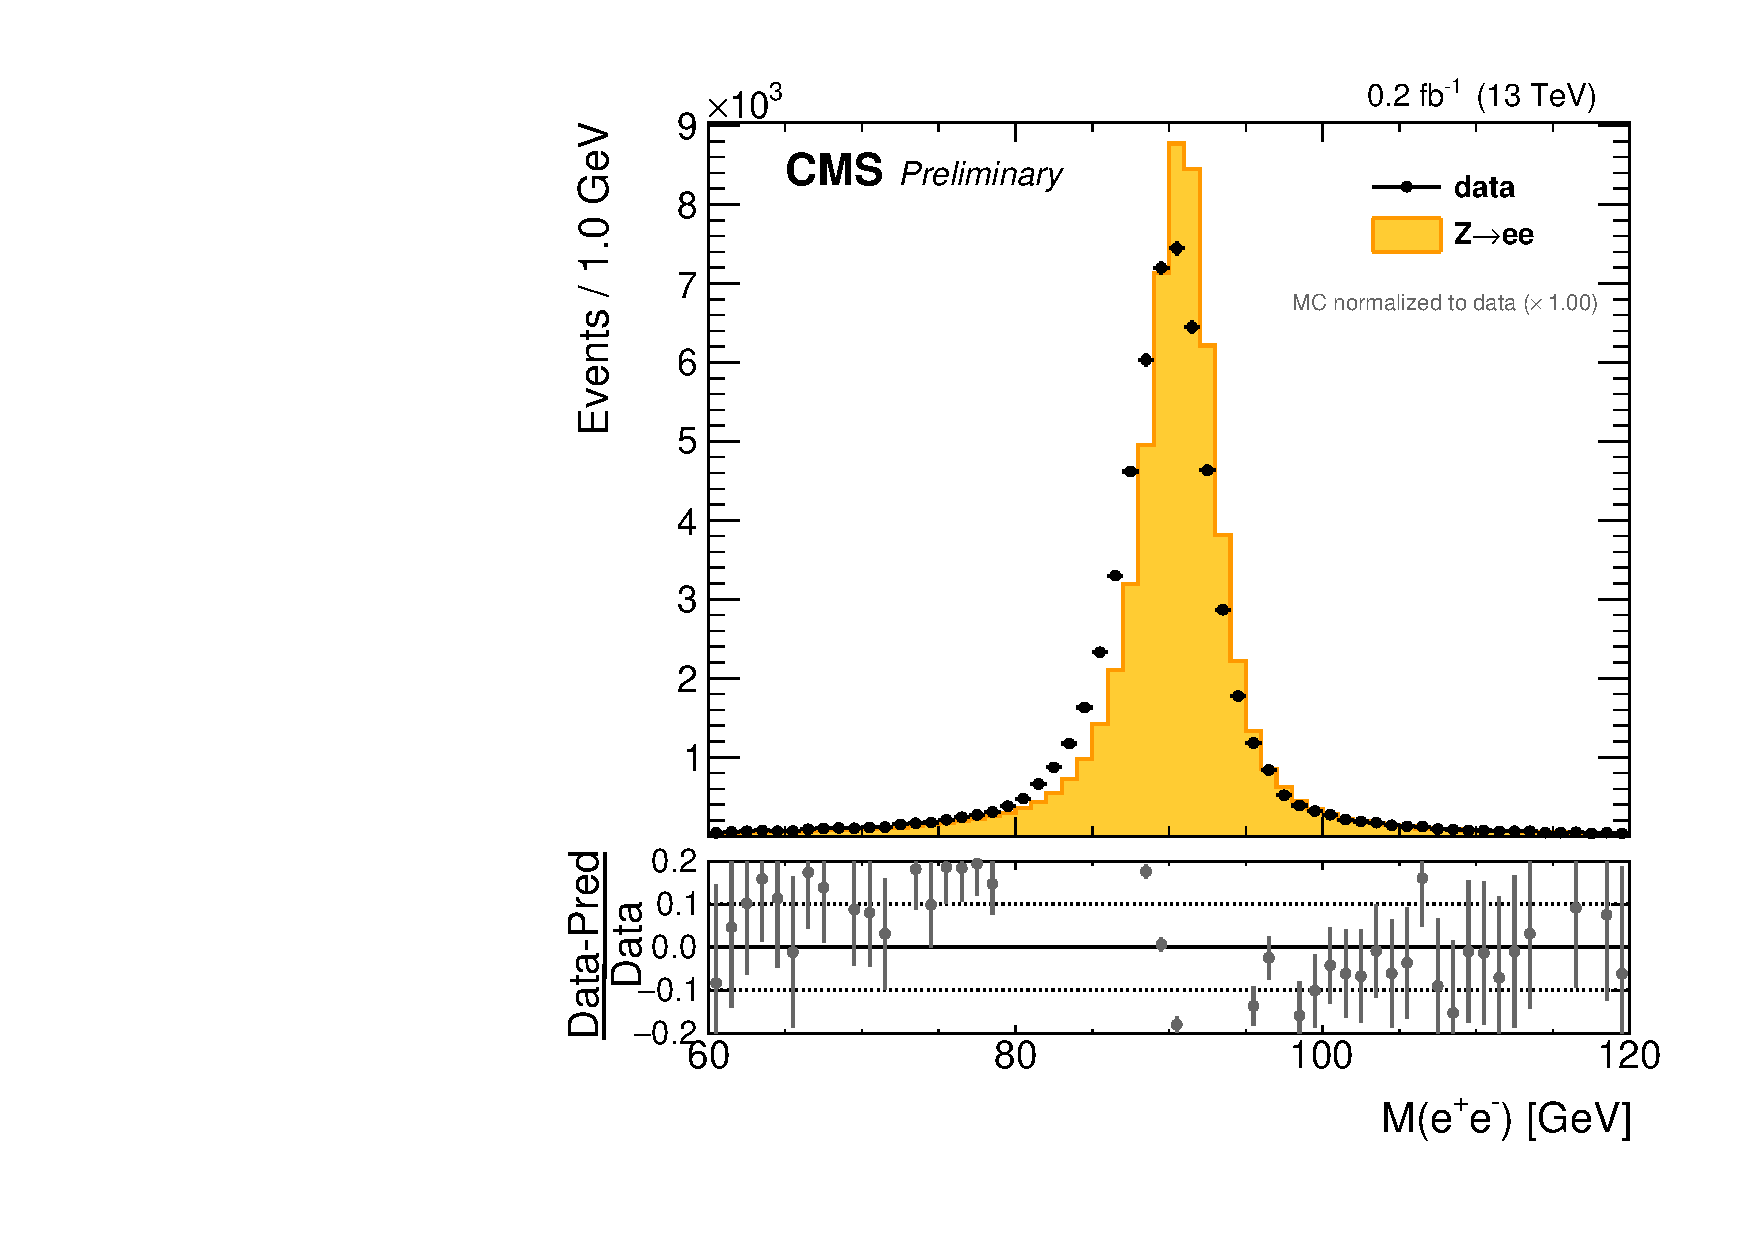
\includegraphics[width=0.49\textwidth]{plots/LepScaleSmear/plotZee13TeV_noCorr/zee_norm.pdf}
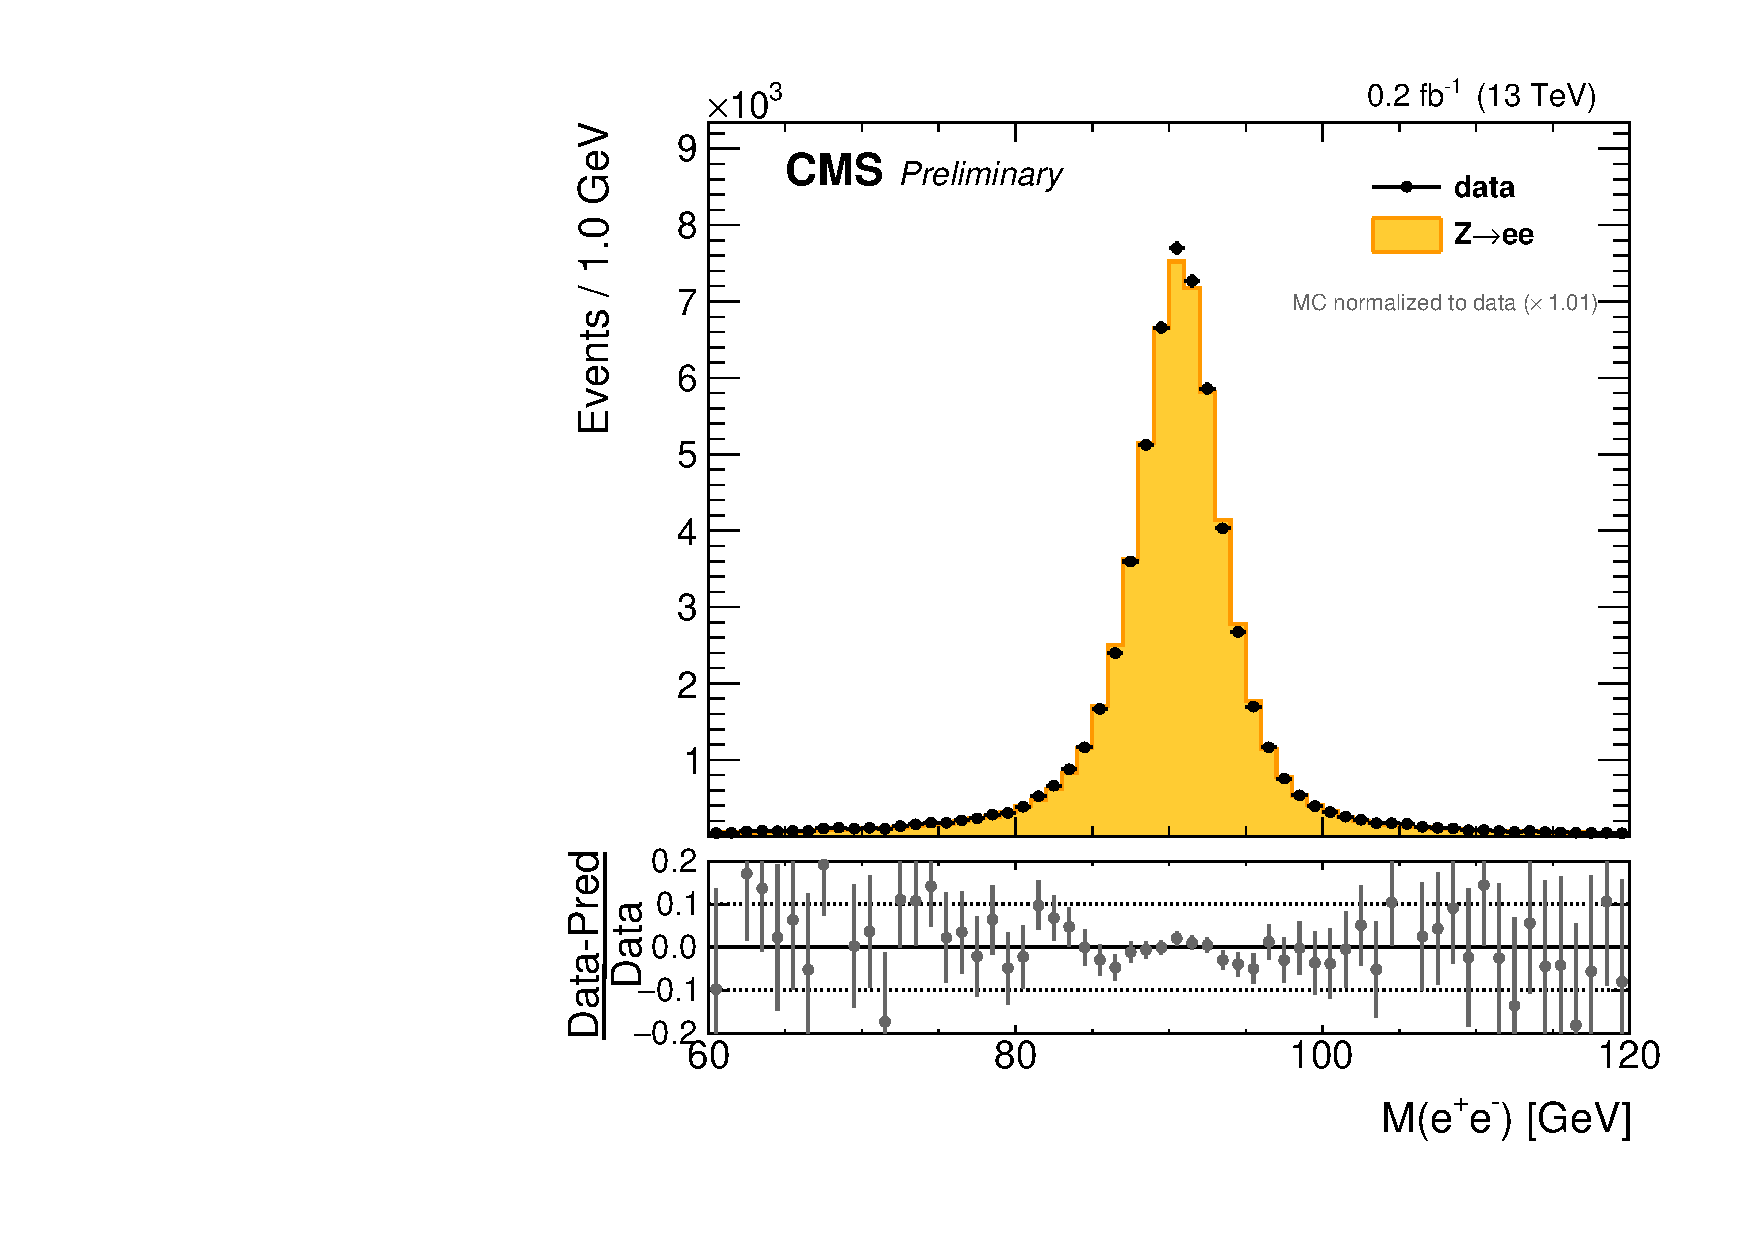
\includegraphics[width=0.49\textwidth]{plots/LepScaleSmear/plotZee13TeV_corr/zee_norm.pdf}
\\
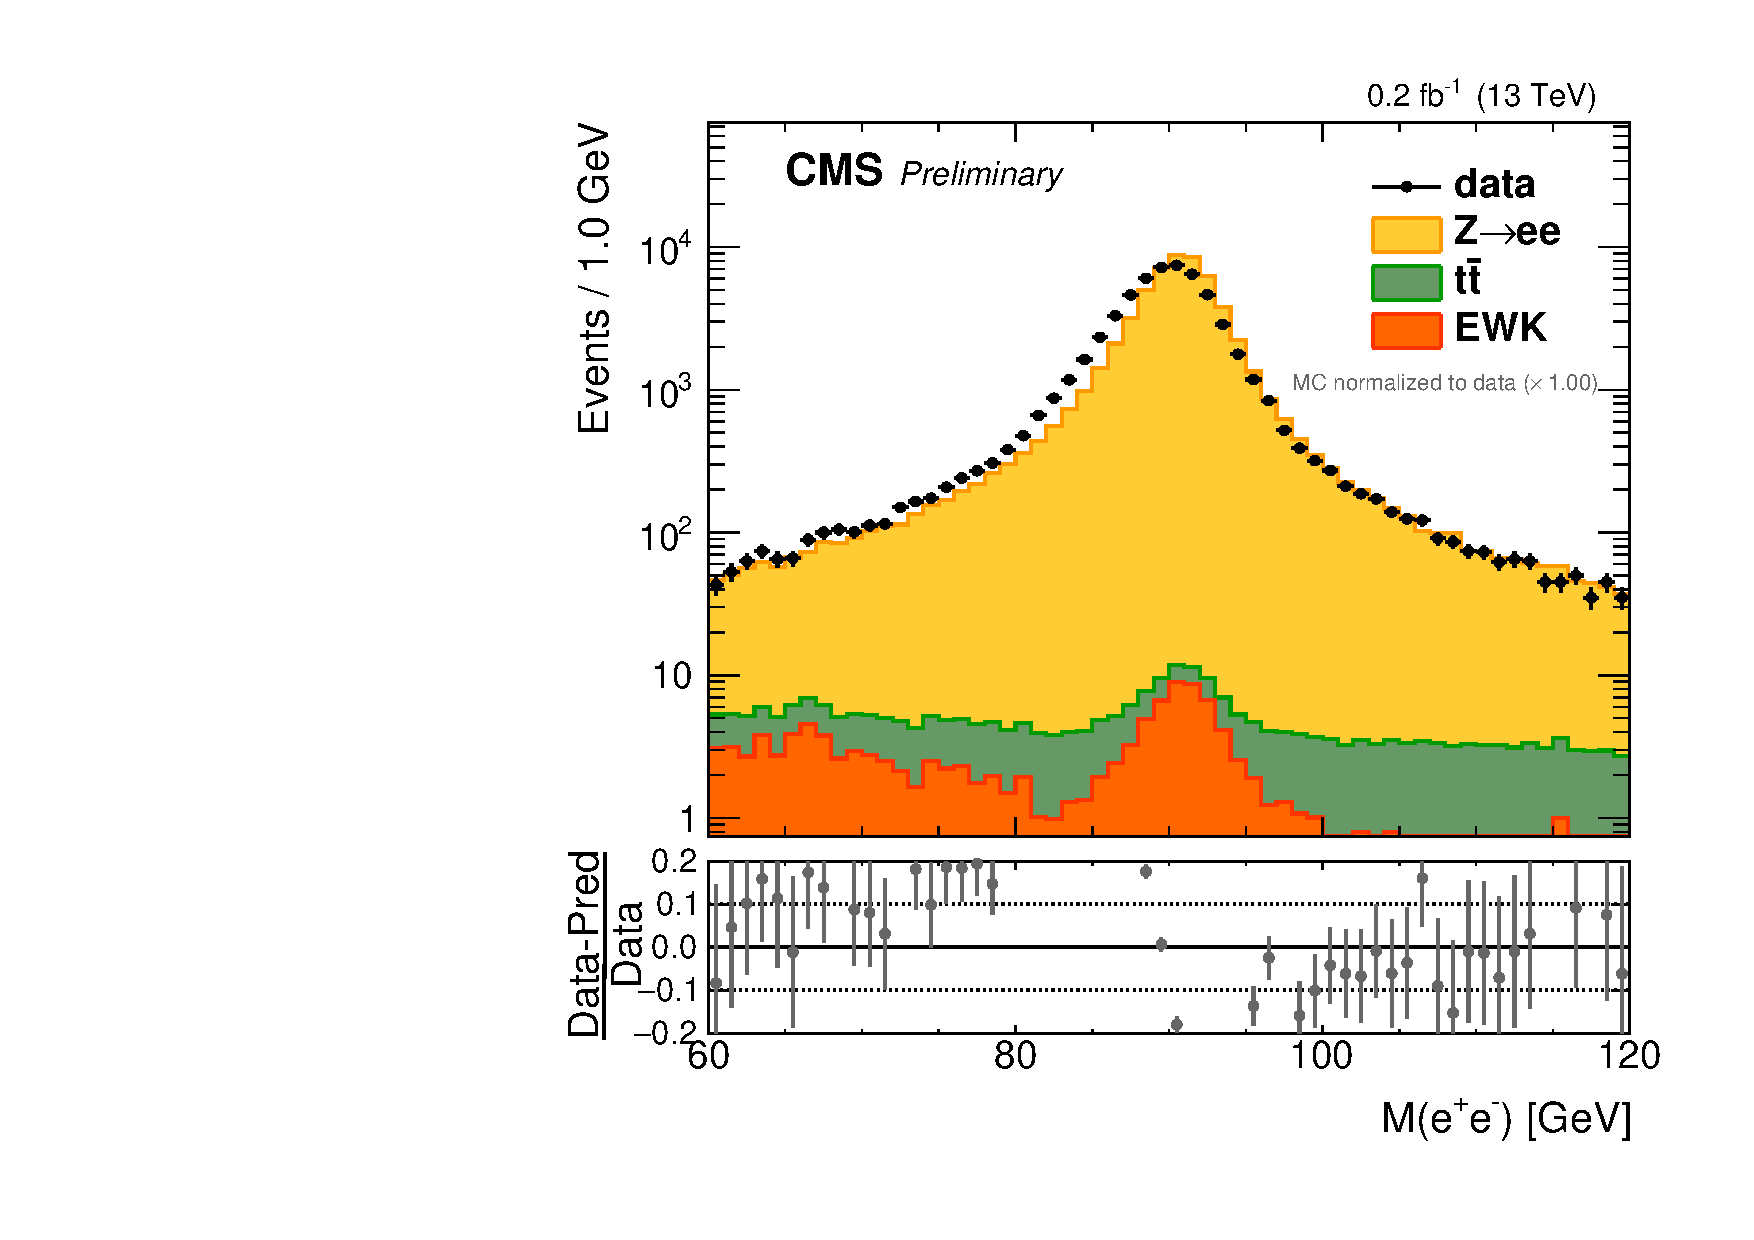
\includegraphics[width=0.49\textwidth]{plots/LepScaleSmear/plotZee13TeV_noCorr/zeelog_norm.pdf}
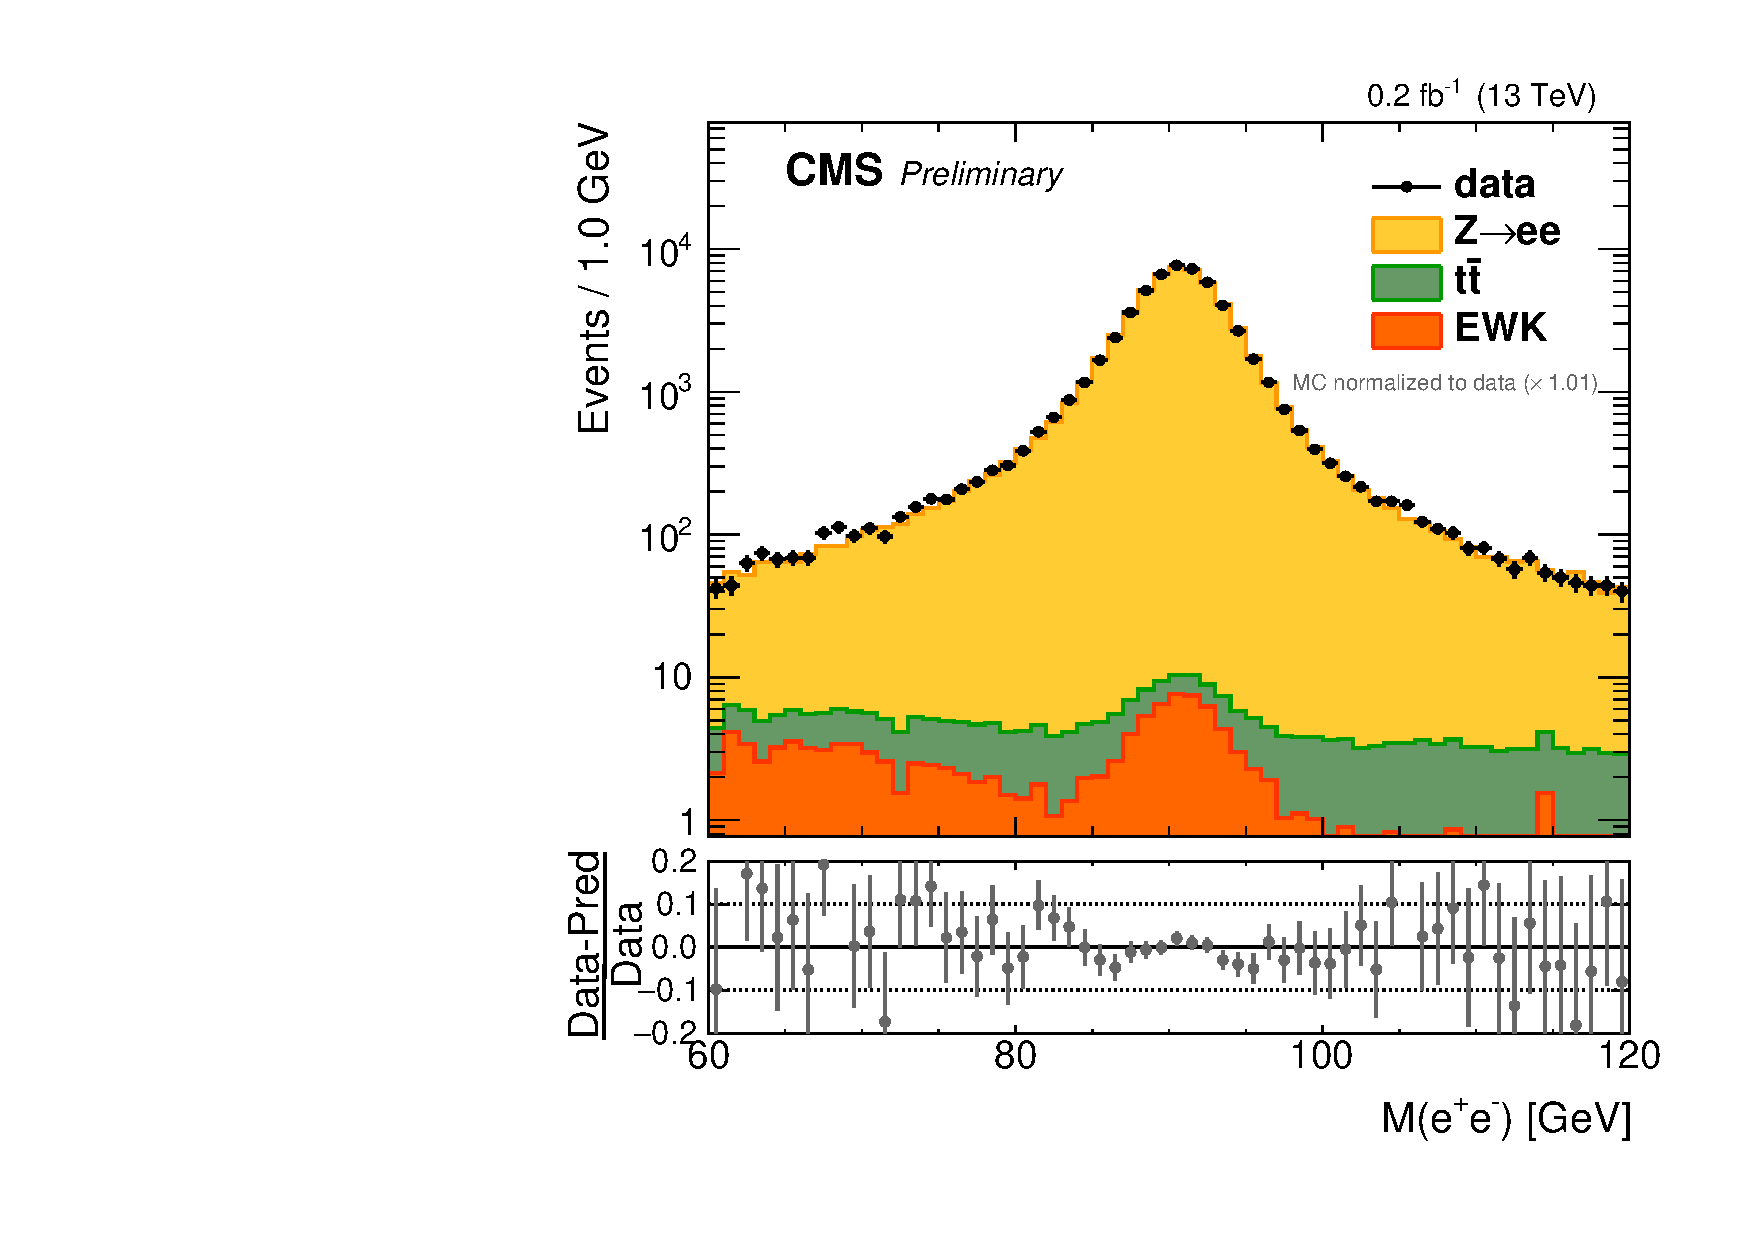
\includegraphics[width=0.49\textwidth]{plots/LepScaleSmear/plotZee13TeV_corr/zeelog_norm.pdf}
\caption{\zee dilepton mass spectrum at \serah, with (right) and without (left) electron energy scale and resolution corrections.}
\label{fig:lepscale:zee:13}
\end{figure}
\begin{figure}[htbp]
\centering
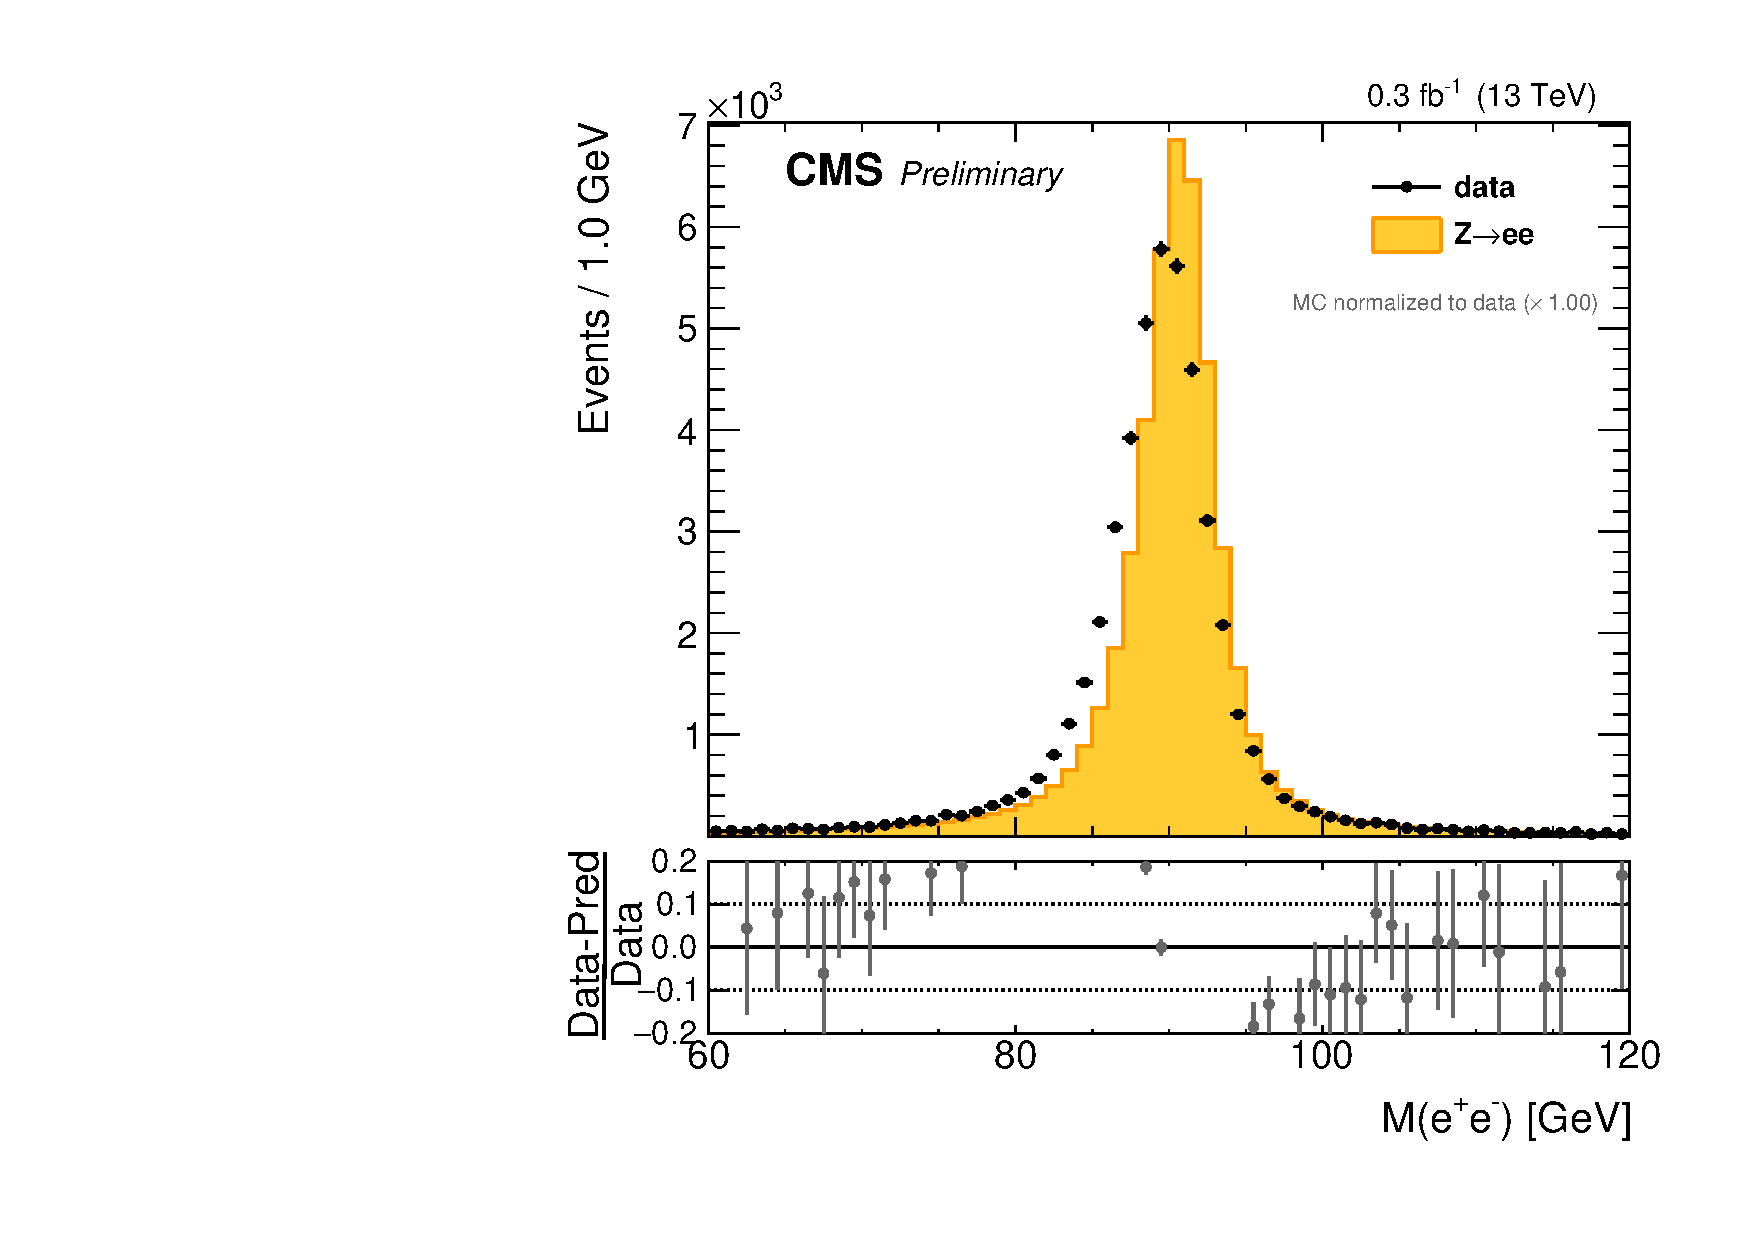
\includegraphics[width=0.49\textwidth]{plots/LepScaleSmear/plotZee5TeV_noCorr/zee_norm.pdf}
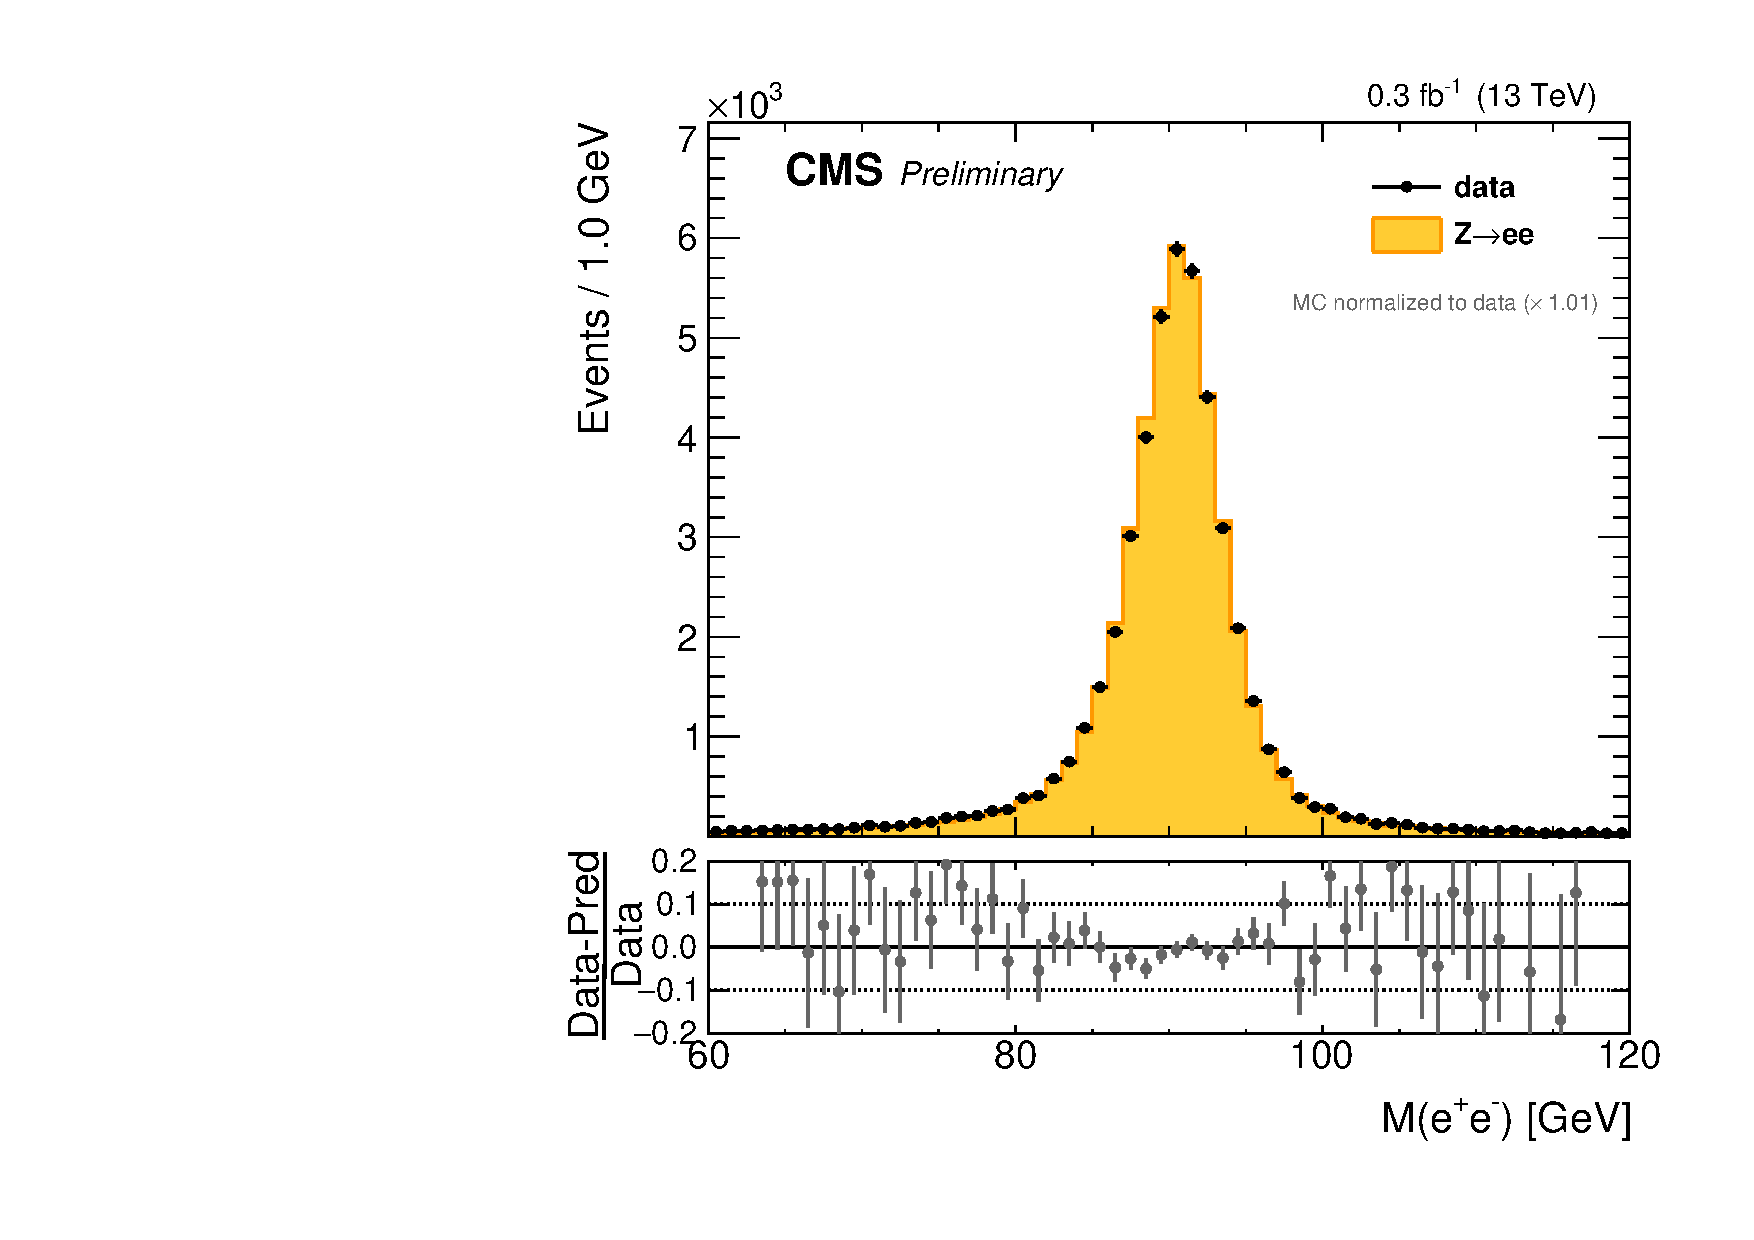
\includegraphics[width=0.49\textwidth]{plots/LepScaleSmear/plotZee5TeV_corr/zee_norm.pdf}
\\
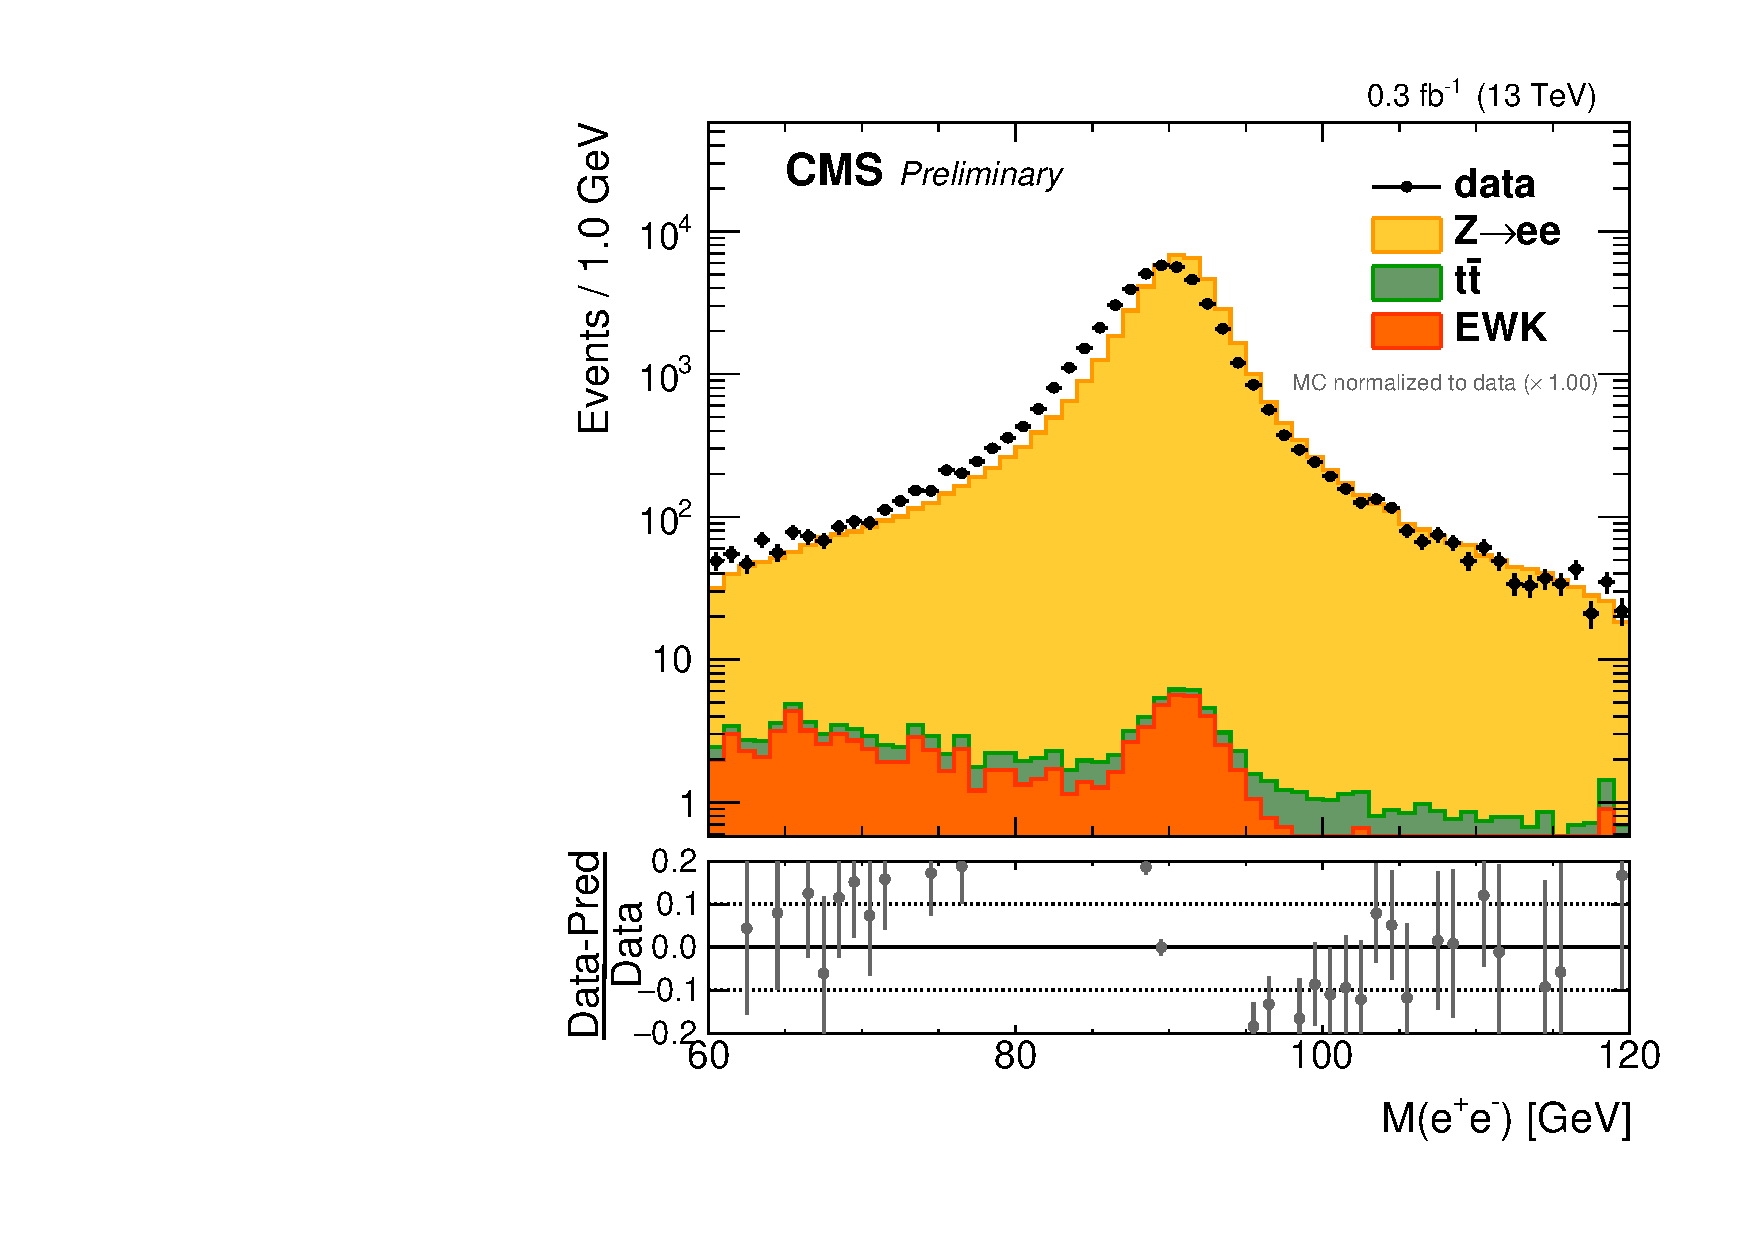
\includegraphics[width=0.49\textwidth]{plots/LepScaleSmear/plotZee5TeV_noCorr/zeelog_norm.pdf}
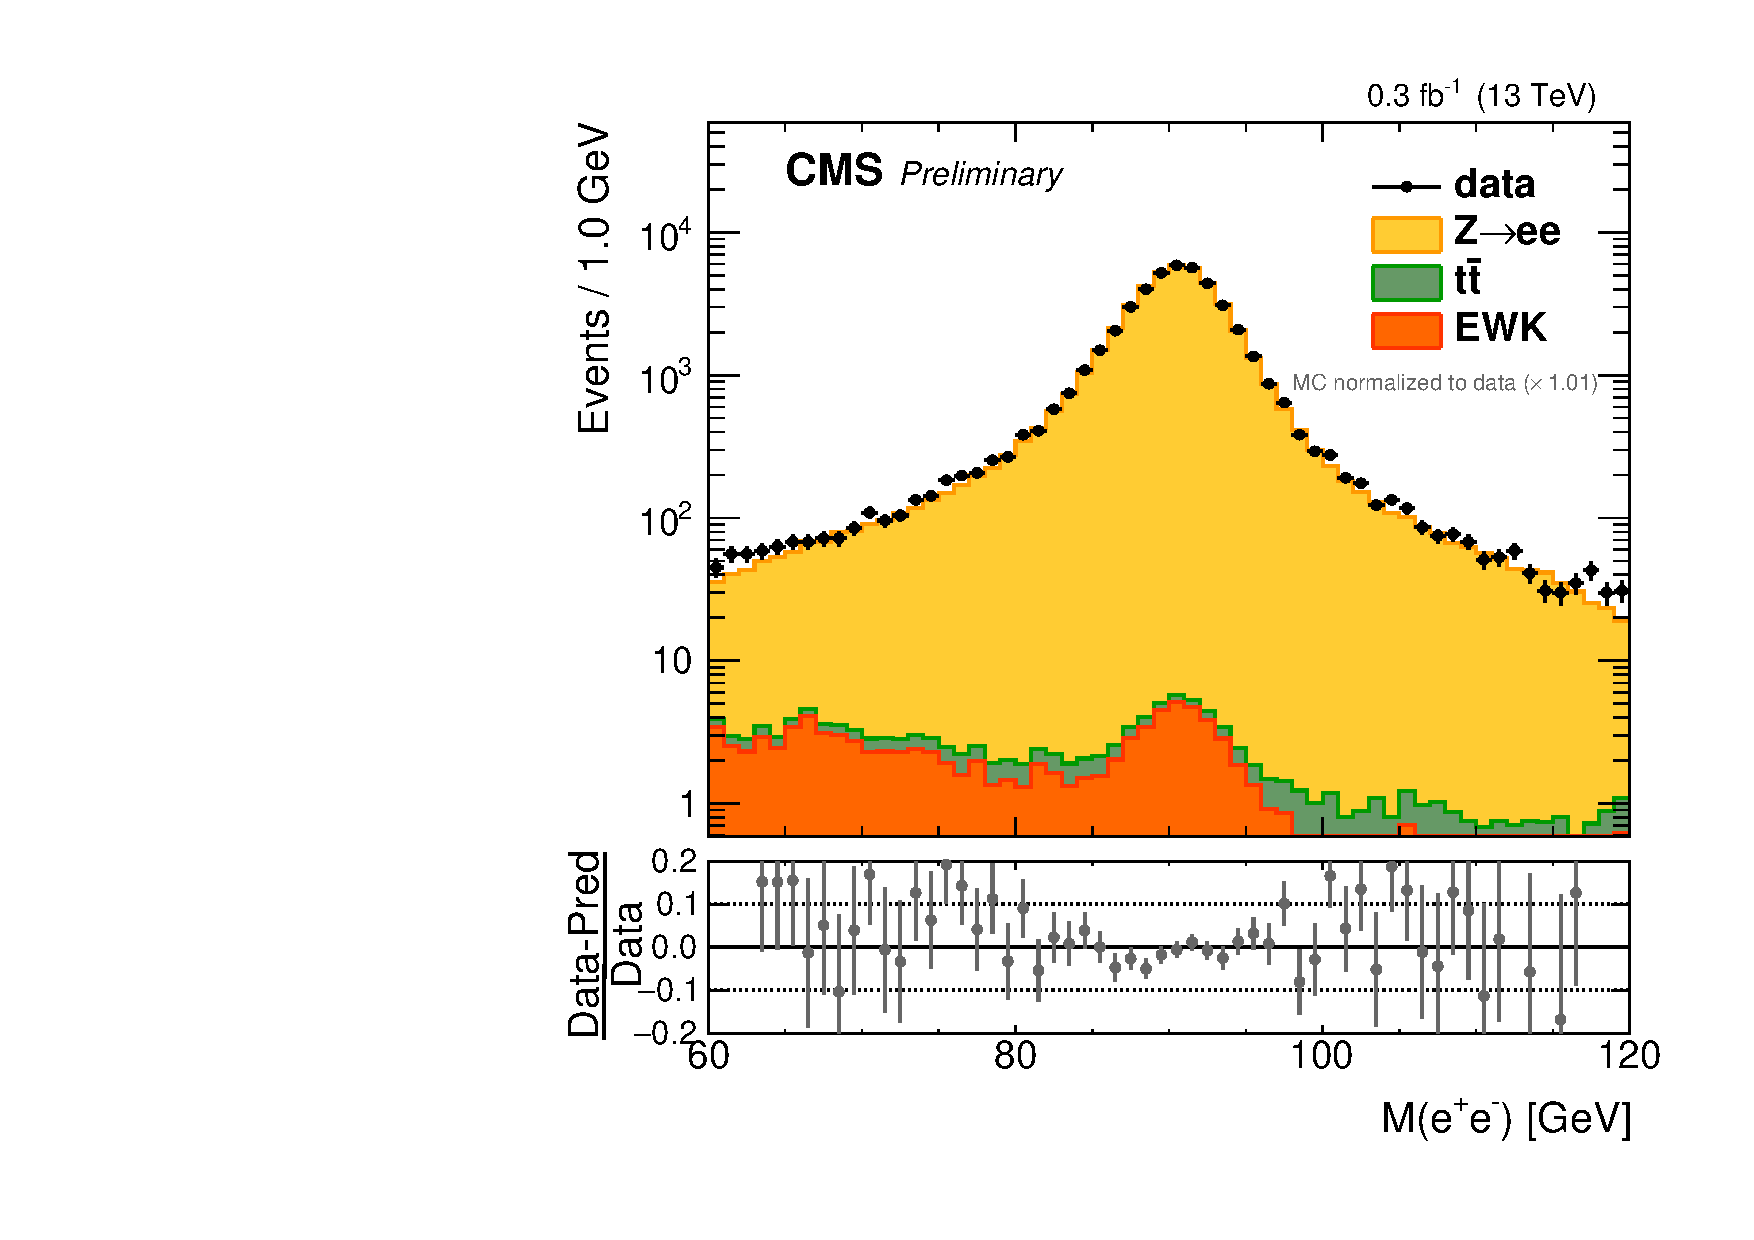
\includegraphics[width=0.49\textwidth]{plots/LepScaleSmear/plotZee5TeV_corr/zeelog_norm.pdf}
\caption{\zee dilepton mass spectrum at \serag, with (right) and without (left) electron energy scale and resolution corrections.}
\label{fig:lepscale:zee:5}
\end{figure}


\subsection{Muon Momentum Corrections}
As with electrons, muon momentum measurements include the need for corrections, though the effect is much smaller than for electrons. Corrections are derived from average lepton \pt and \zmm invariant mass distribution, so that the maximum and width of the \zmm invariant mass in simulation matches data\cite{Bodek:2012id}.  A single set of corrections is used for the entirety of 2017 data-taking. Distributions of \zmm \mll before and after applying muon momentum corrections are shown in Figure~\ref{fig:lepscale:zmm:5} (Figure~\ref{fig:lepscale:zmm:13}) for \sg (\sh).

\begin{figure}[htbp]
\centering
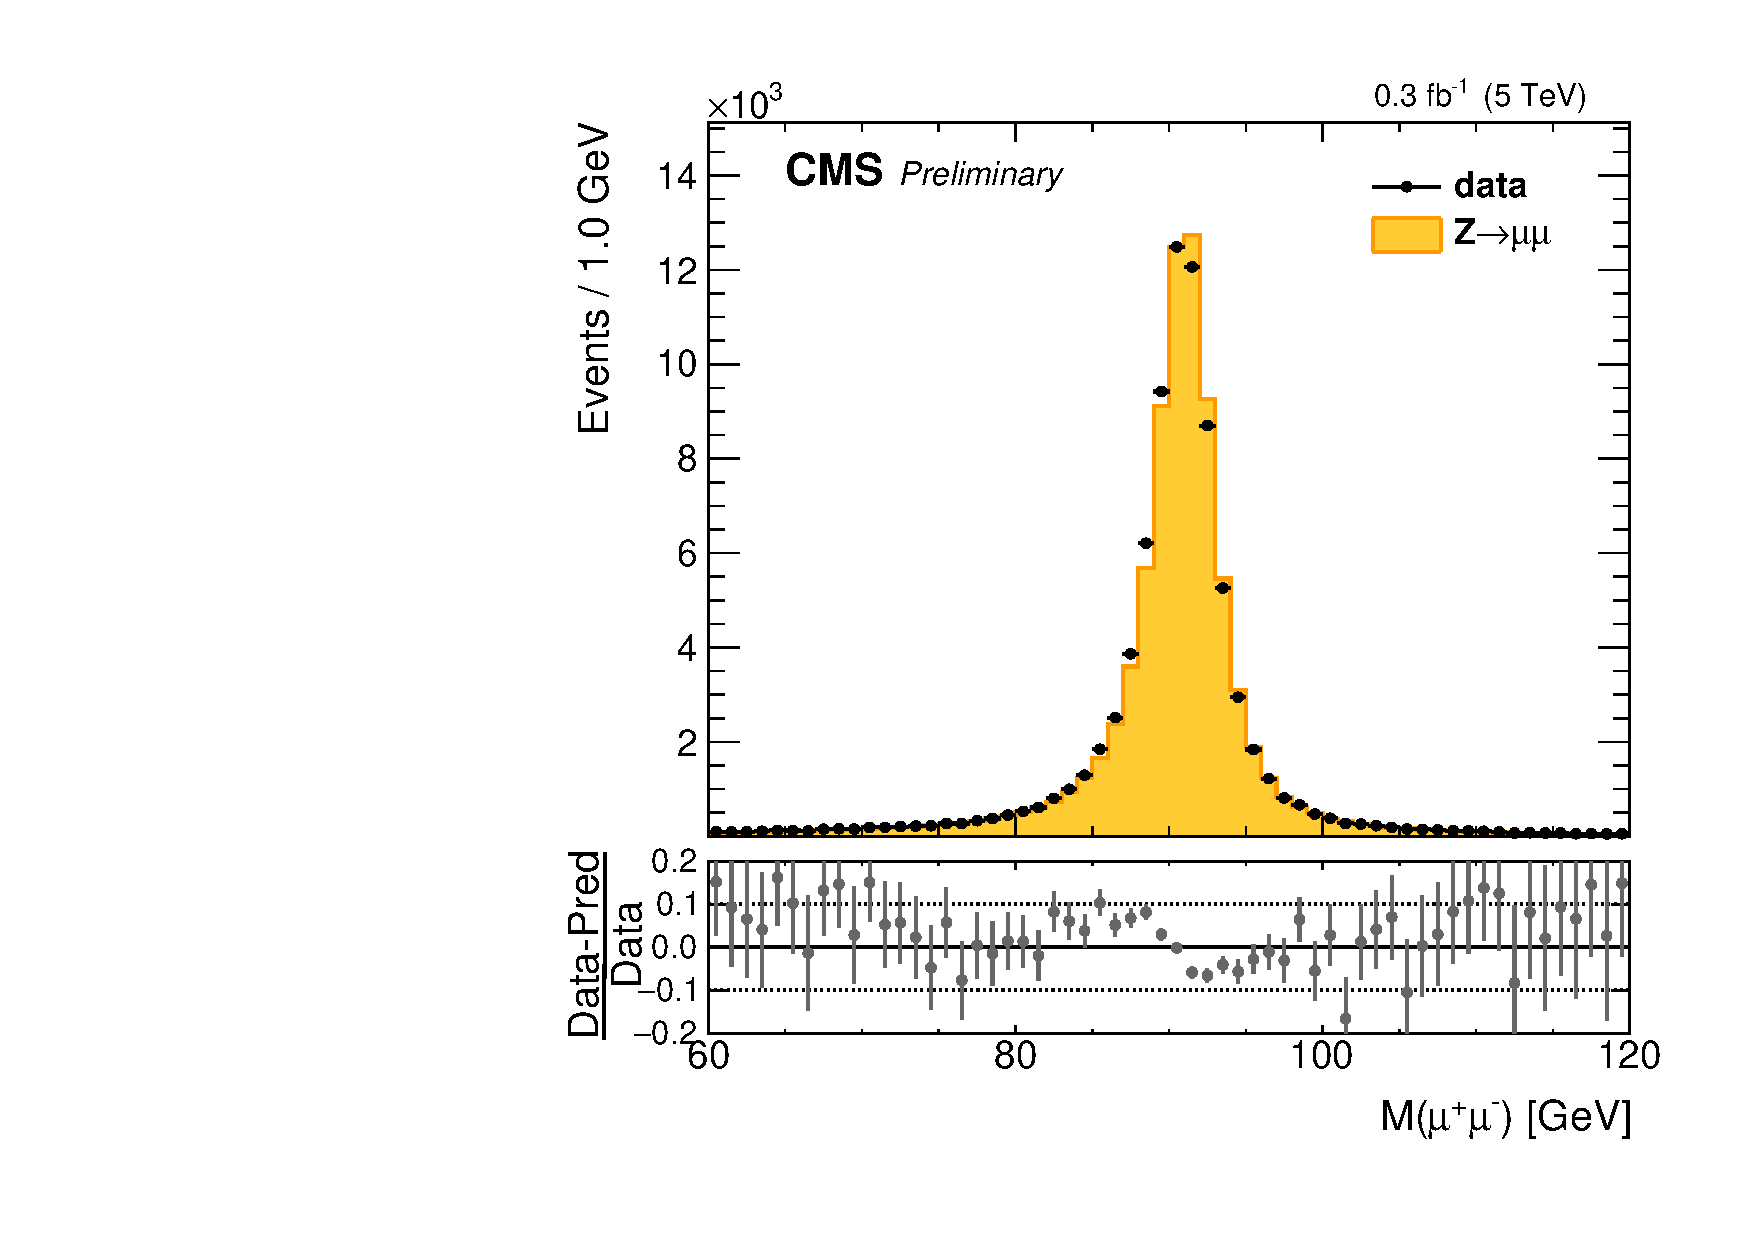
\includegraphics[width=0.49\textwidth]{plots/LepScaleSmear/plotZmm5TeV_noCorr/zmm.pdf}
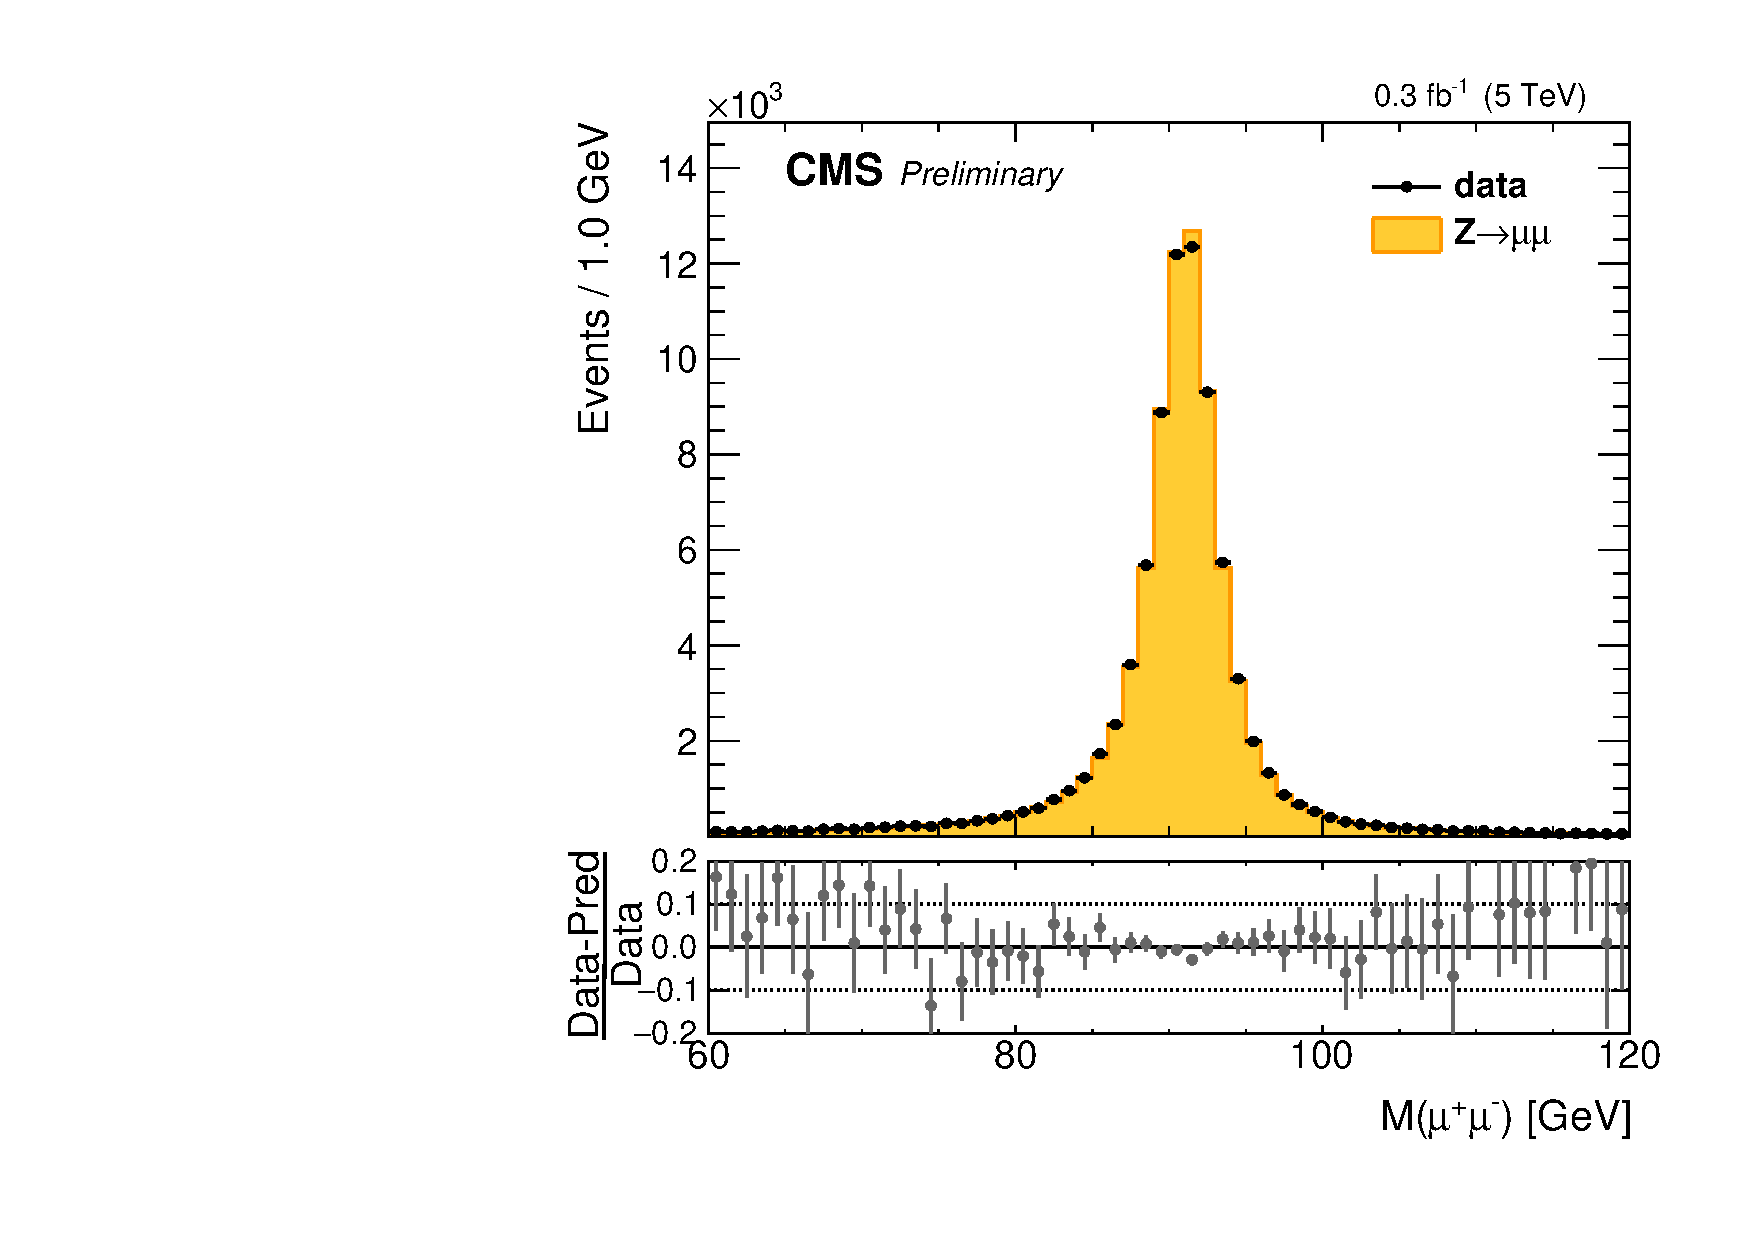
\includegraphics[width=0.49\textwidth]{plots/LepScaleSmear/plotZmm5TeV_corr/zmm.pdf}
\\
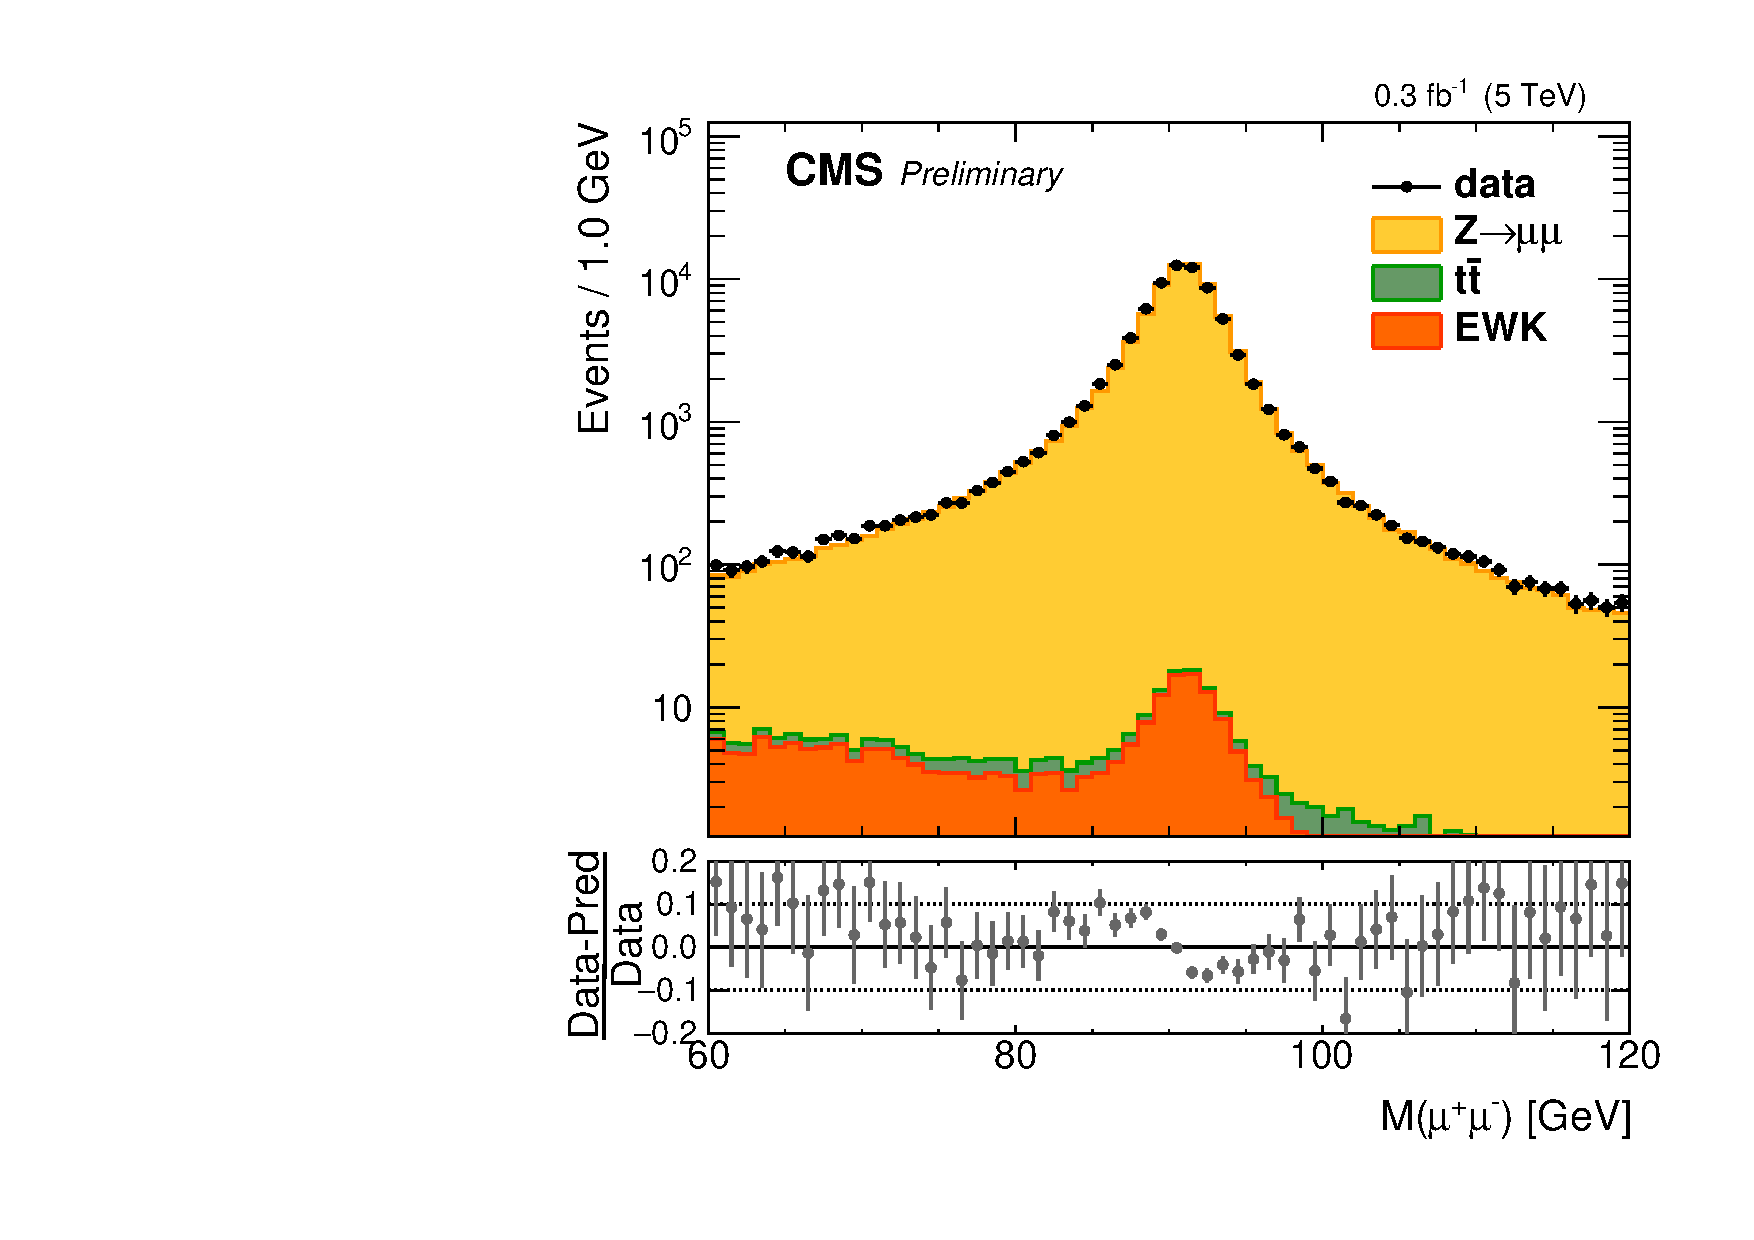
\includegraphics[width=0.49\textwidth]{plots/LepScaleSmear/plotZmm5TeV_noCorr/zmmlog.pdf}
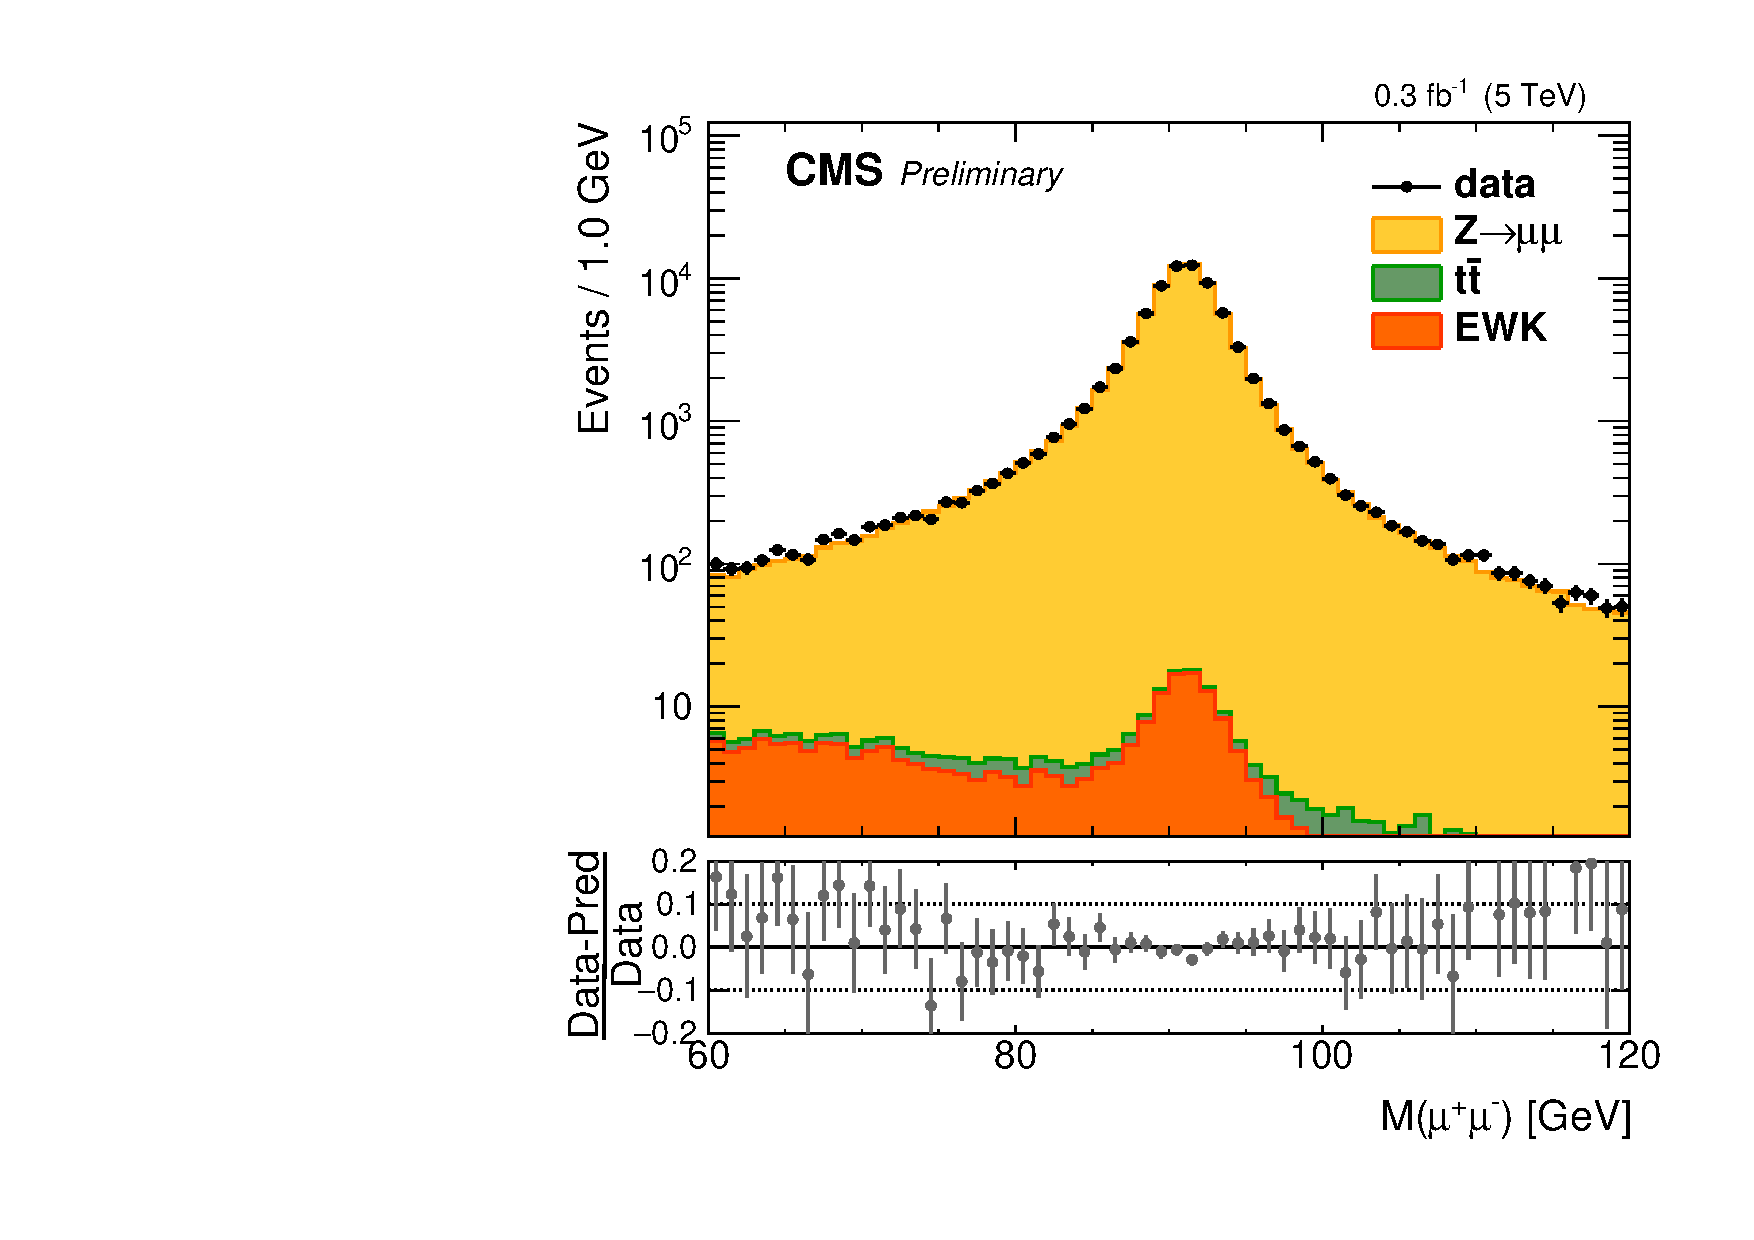
\includegraphics[width=0.49\textwidth]{plots/LepScaleSmear/plotZmm5TeV_corr/zmmlog.pdf}
\caption{\zmm dilepton mass spectrum at \sg, with (right) and without (left) muon Rochester corrections.}
\label{fig:lepscale:zmm:5}
\end{figure}
\begin{figure}[htbp]
\centering
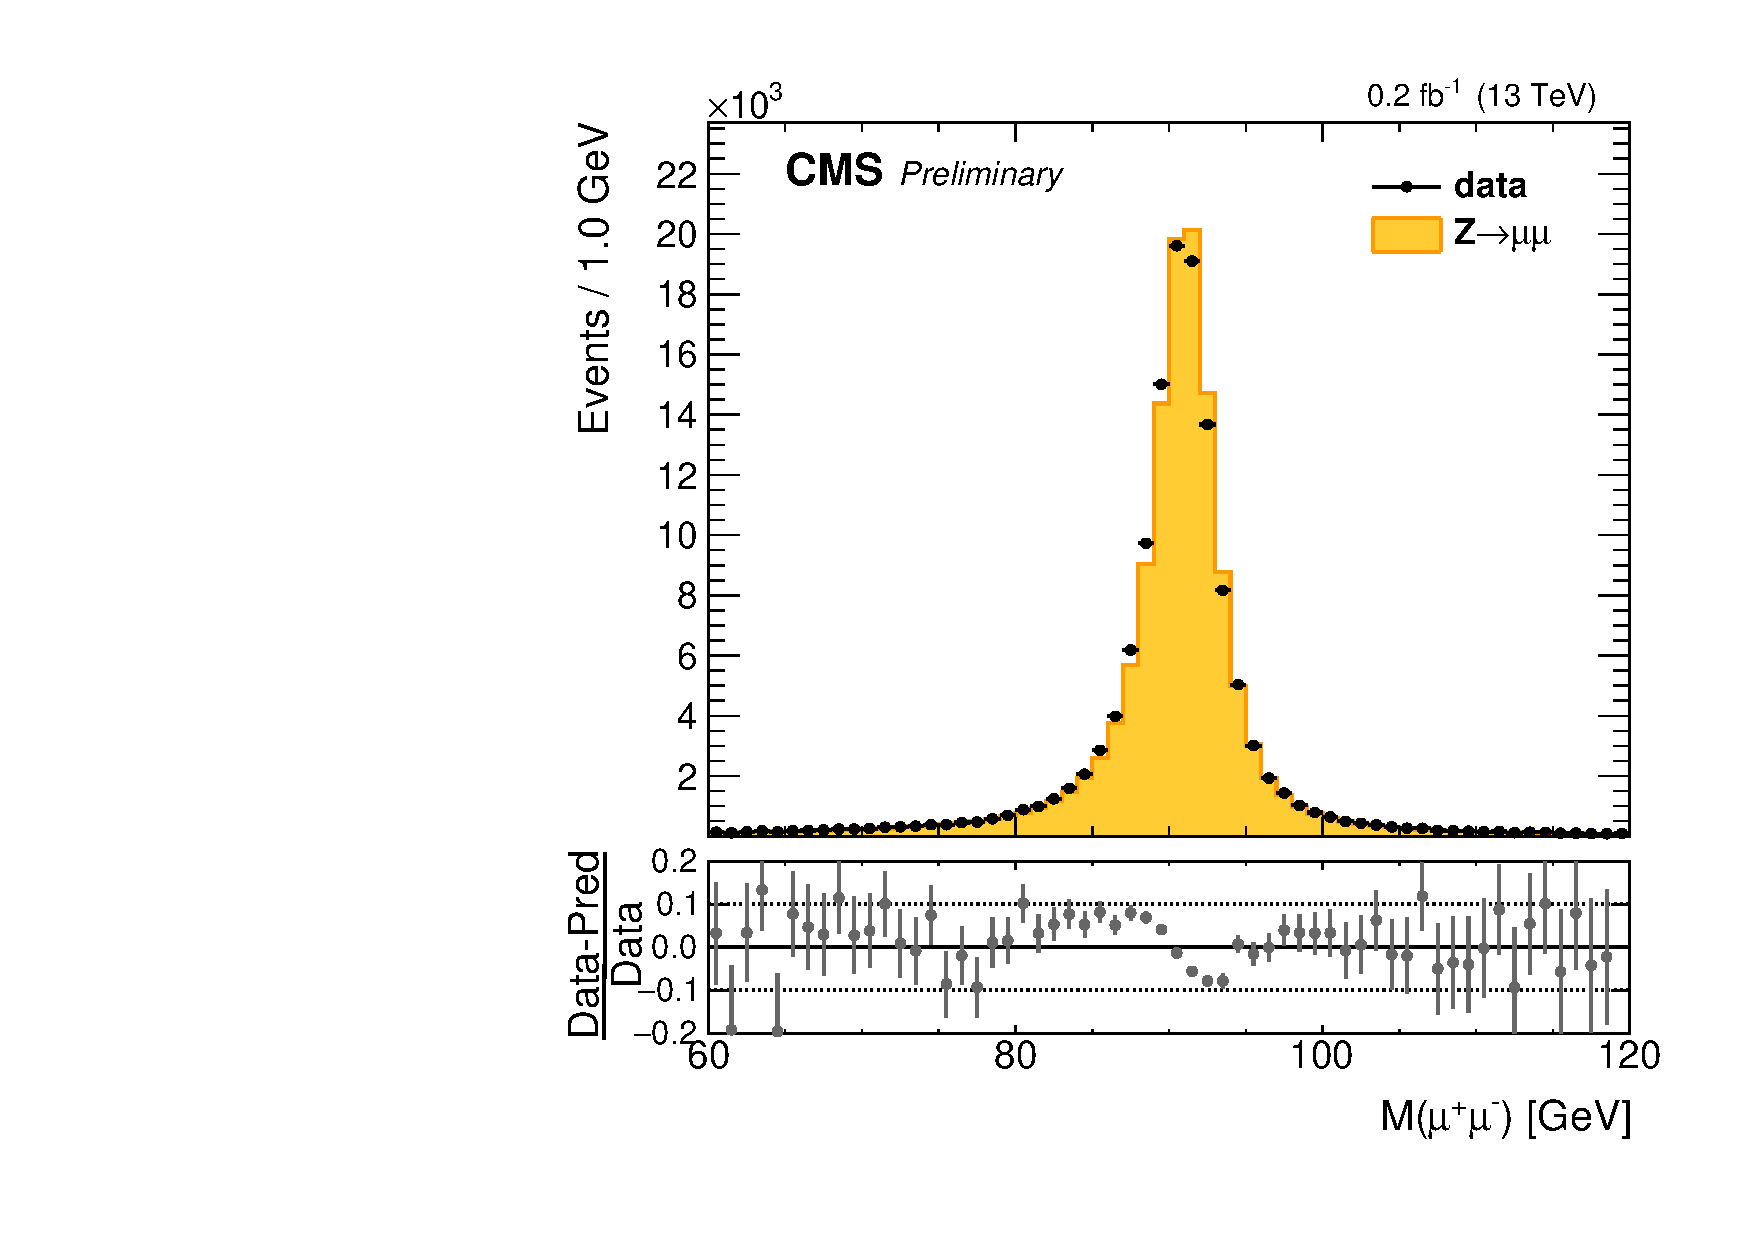
\includegraphics[width=0.49\textwidth]{plots/LepScaleSmear/plotZmm13TeV_noCorr/zmm.pdf}
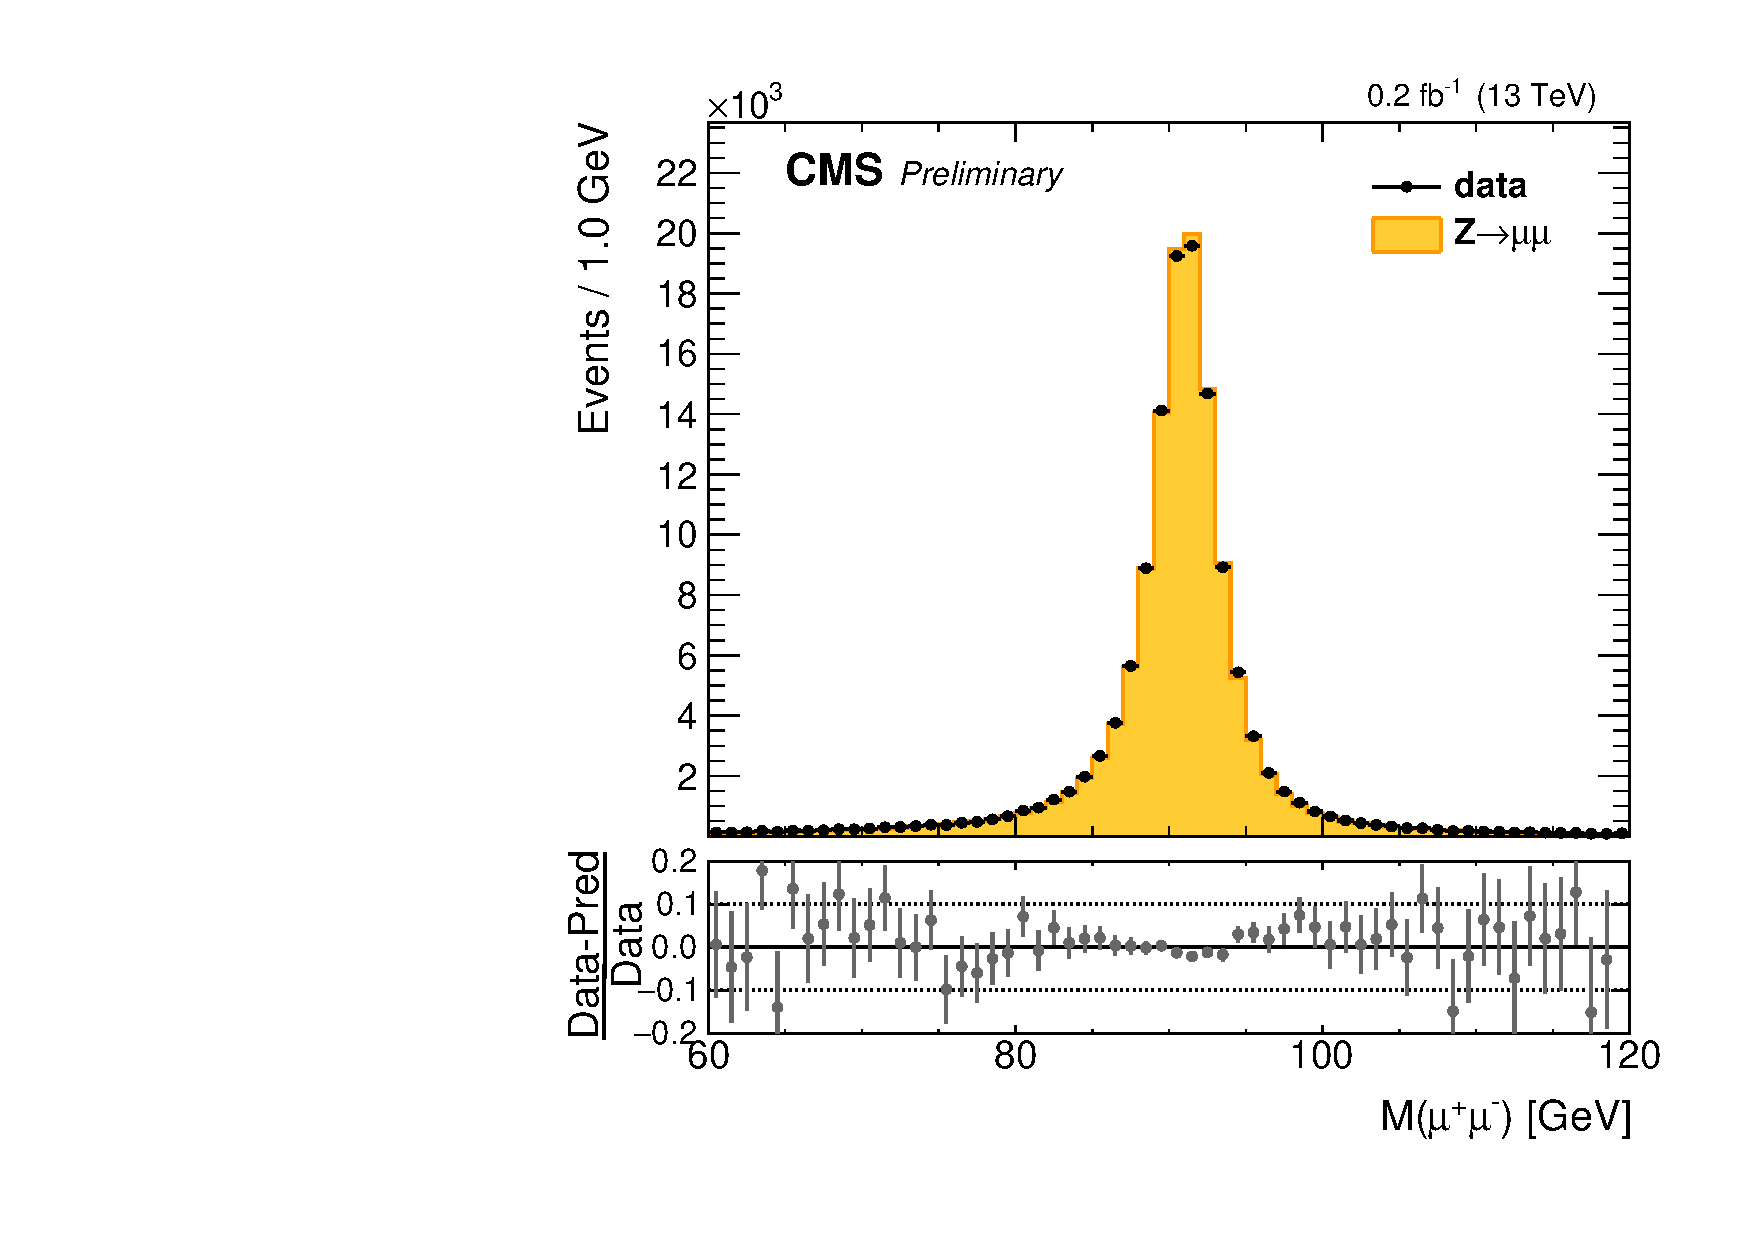
\includegraphics[width=0.49\textwidth]{plots/LepScaleSmear/plotZmm13TeV_corr/zmm.pdf}
\\
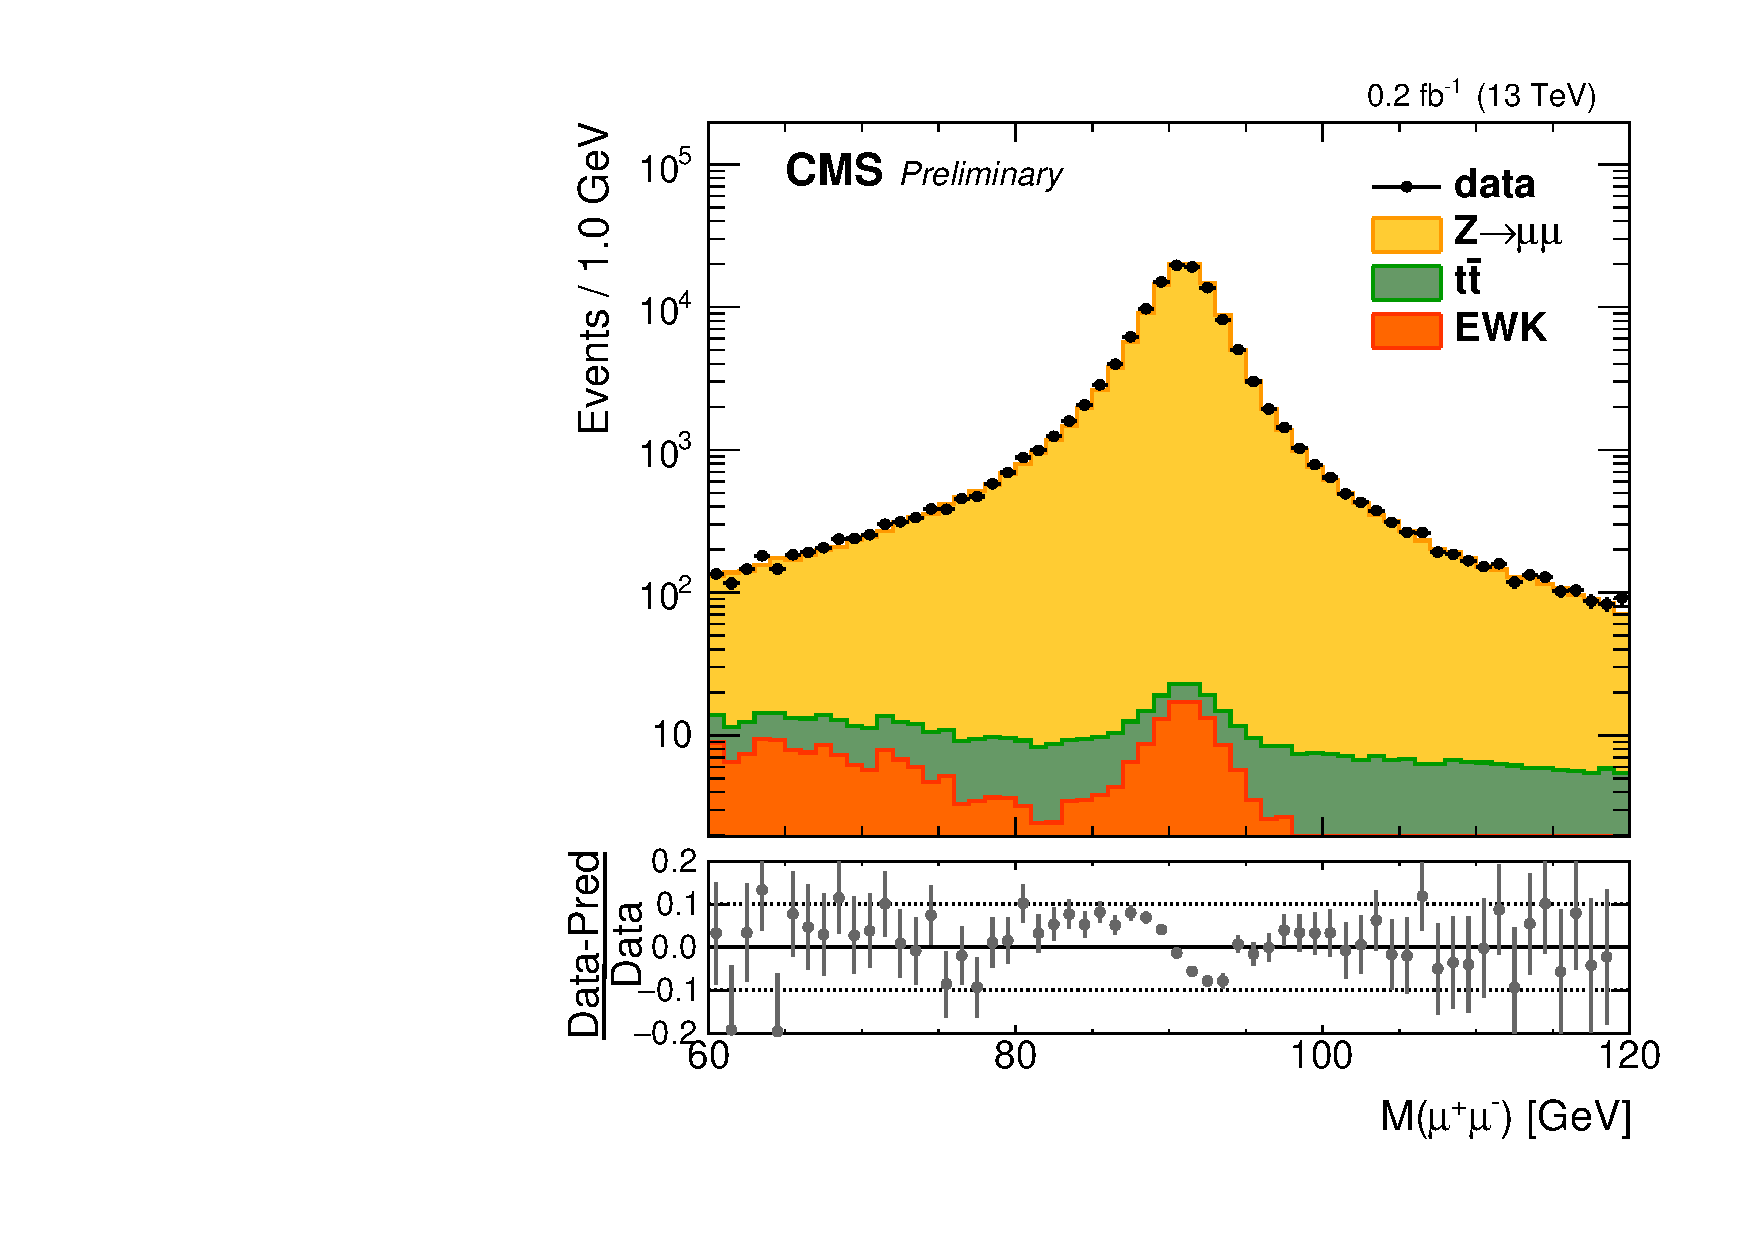
\includegraphics[width=0.49\textwidth]{plots/LepScaleSmear/plotZmm13TeV_noCorr/zmmlog.pdf}
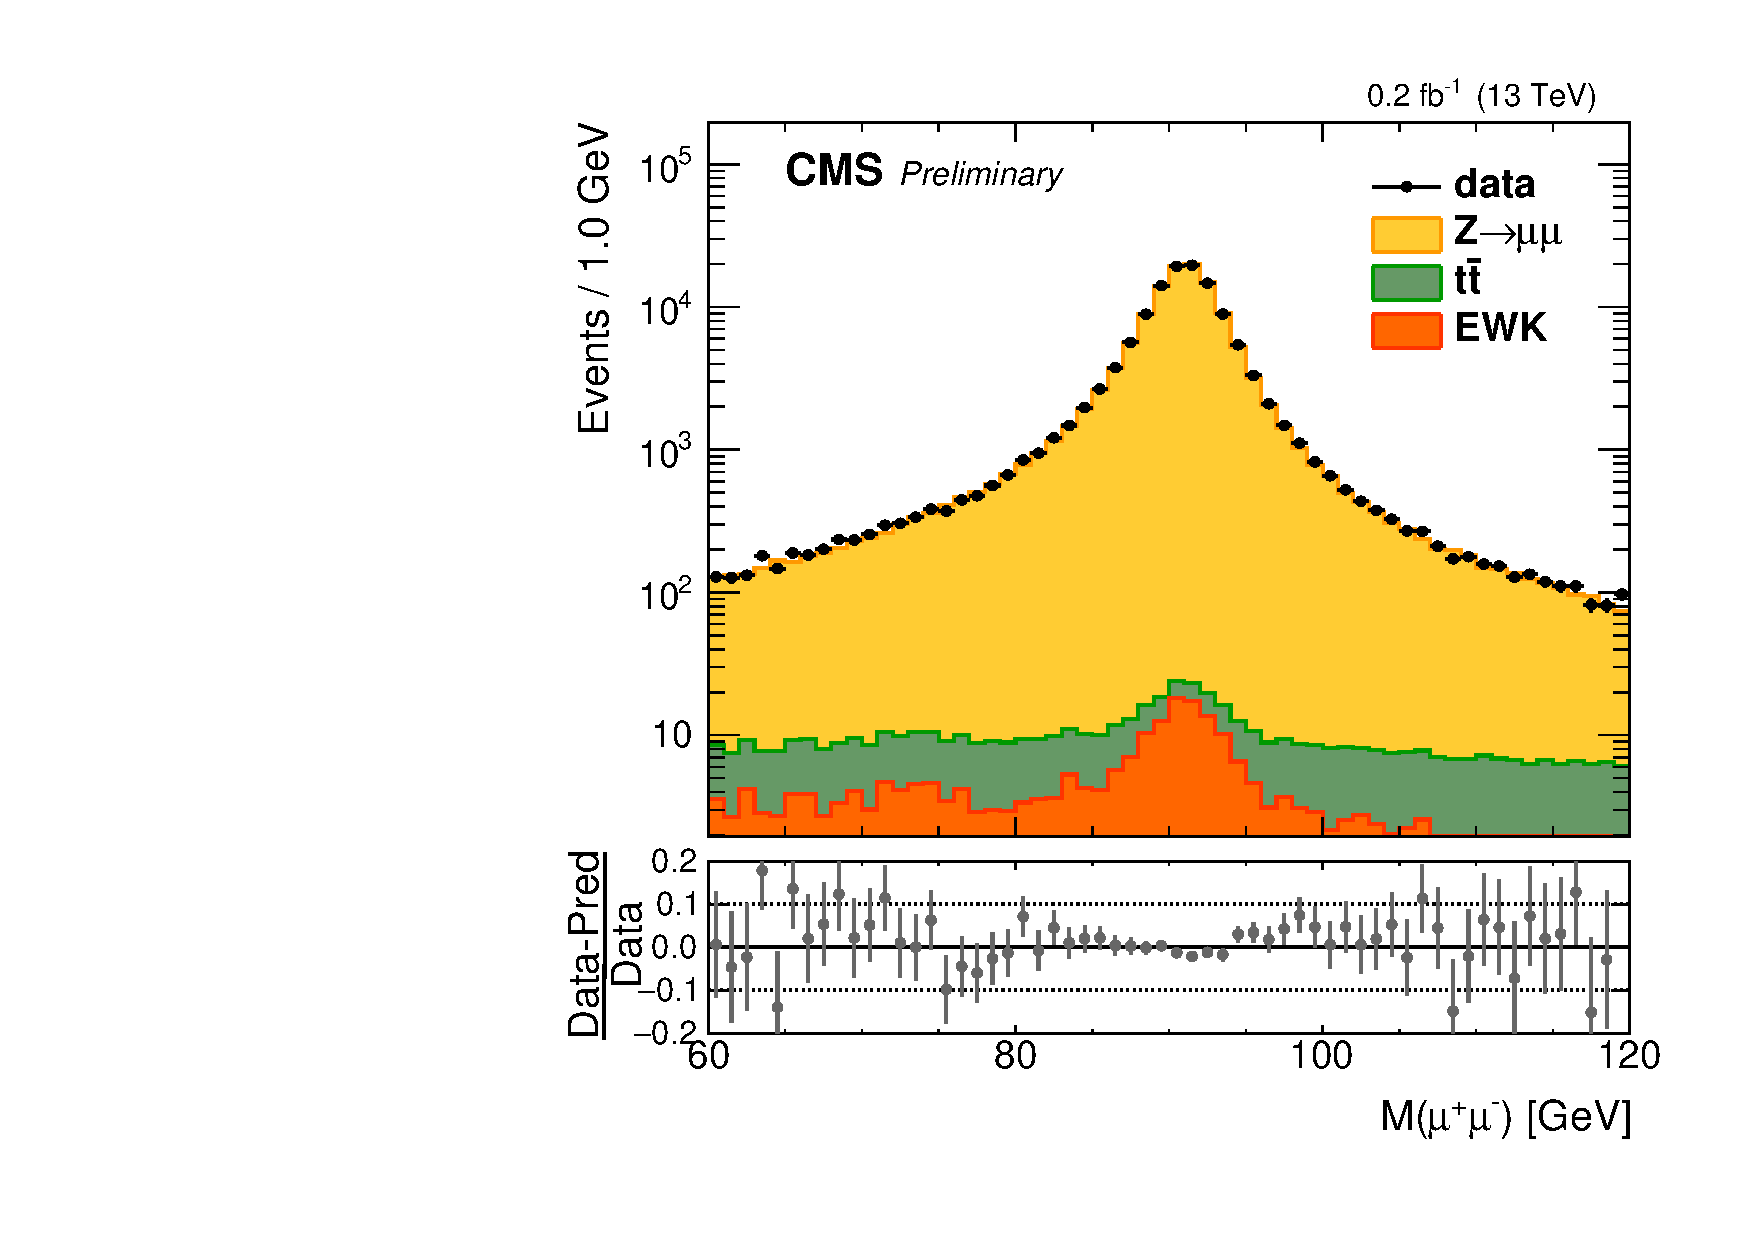
\includegraphics[width=0.49\textwidth]{plots/LepScaleSmear/plotZmm13TeV_corr/zmmlog.pdf}
\caption{\zmm dilepton mass spectrum at \sh, with (right) and without (left) muon momentum corrections.}
\label{fig:lepscale:zmm:13}
\end{figure}


%%%%%%%%%%%%%%%%%%%%%%%%%%%%%%%%%%%%%%%%%%%%
%                Prefiring

\section{ECAL L1 Trigger Prefiring}\label{ch:prefire}

Radiation damage to the $\mathrm{PbWO_4}$ crystals in the ECAL result in color centers forming within the crystal lattice, reducing transparency and altering light propagation through the crystal. Corrections to accommodate the change in scintillation light transmission were not applied in a way which completely removed the timing drift. Trigger primitives (TPs) in the forward regions of ECAL, $2.0 < |\eta| < 3.5$, were affected by the timing drift during the 2017 data-taking period. The timing drift caused certain TPs in the forward ECAL region to be incorrectly associated with the wrong bunch crossing, an effect described as "prefiring". The global trigger rules disallow the collection of consecutive bunch crossings, and no more than one event accepted per three consecutive bunch crossings, so an event which contains a prefired trigger primitive will cause the BX-1 (previous bunch crossing) to be read out, while BX0 (the current one containing the actual event with the TP) to be discarded by the trigger. In all likelihood, the read out event will not pass the HLT and will ultimately be discarded.
This effect is not described in simulation, but a correction factor describing the rate of event loss is derived from data. Due to their large EM activity, photons and jets are used as the basis for the prefiring rate descriptions. A prefiring probability is assigned to each simulated event, based on the kinematics of the photons and jets present in the event, in Equation~\ref{eq:prefiring_weight}, re-scales contribution of simulated events given the likelihood of prefiring.
\phil{there is some garbled english please rewrite end of this paragraph also below}.

\begin{figure}[htbp]
\centering
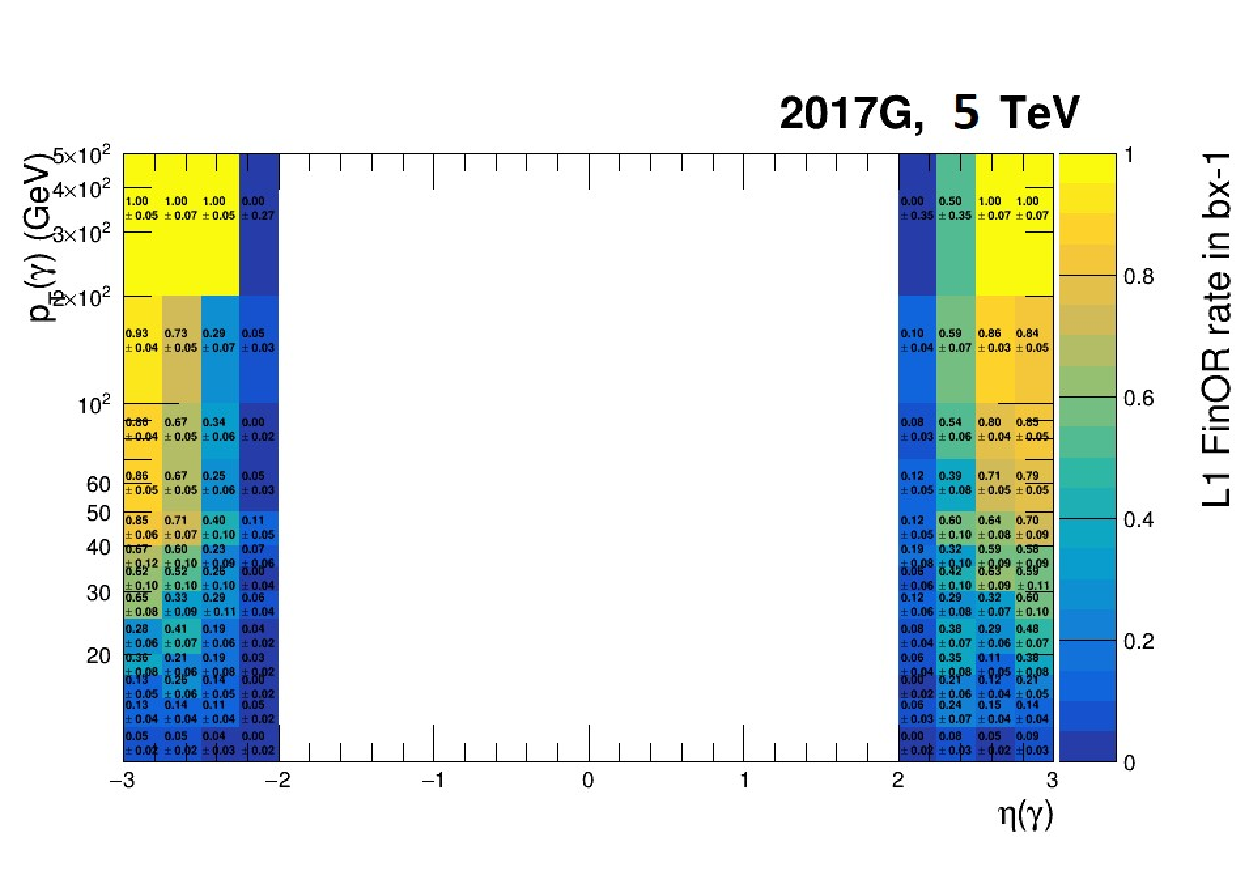
\includegraphics[width=0.49\textwidth]{plots/Prefire/L1prefiring_photonpt_2017G.pdf}
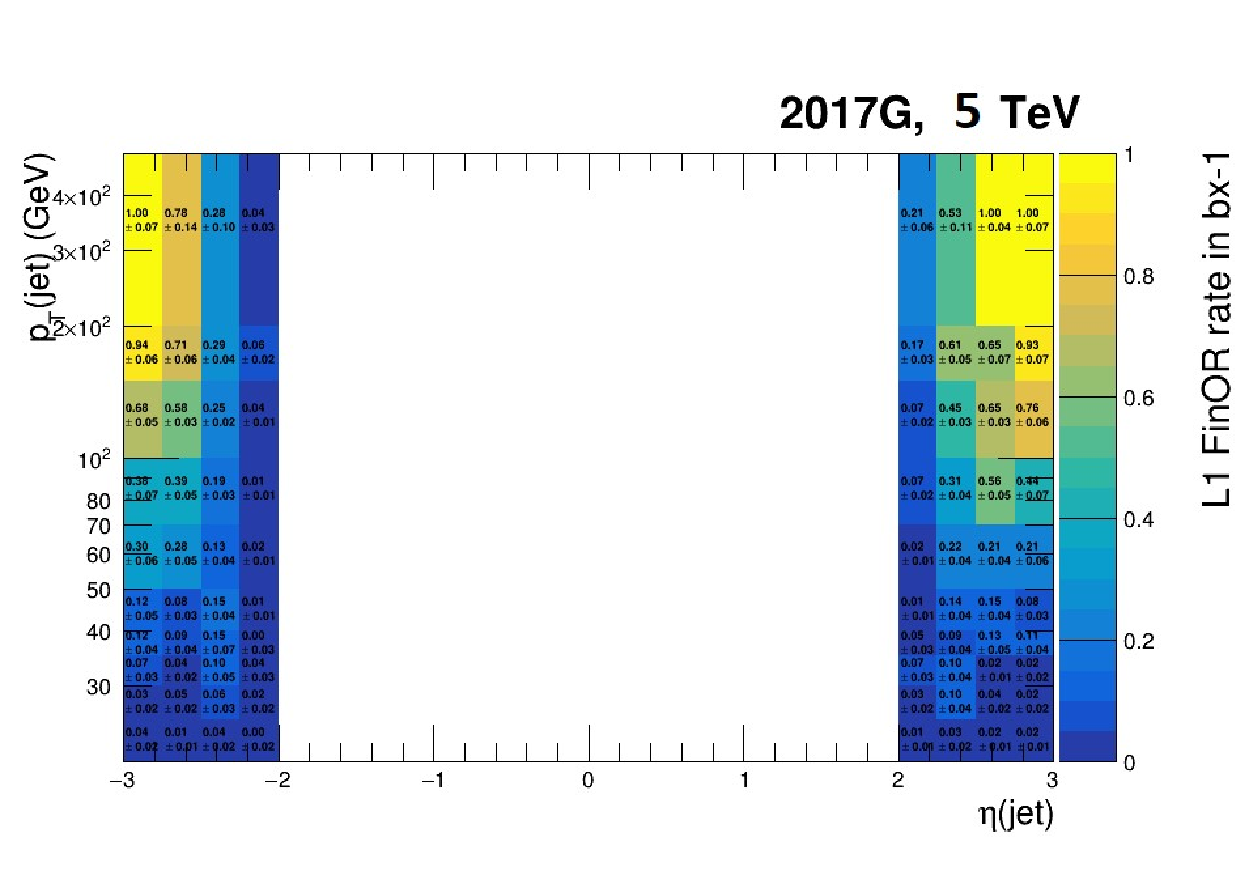
\includegraphics[width=0.49\textwidth]{plots/Prefire/L1prefiring_jetpt_2017G.pdf}
\caption{Pre-firing probability maps for photons (left) and jets (right) for 2017G (\sg). The $z-\mathrm{axis}$ represents the probability of an object with $(\pt,\eta)$ causing pre-firing. Objects with higher \pt and $|\eta| \sim 3$ are more likely to cause pre-firing. Objects with $|\eta| < 2$ do not cause pre-firing.}
\label{fig:prefire:2017G}
\end{figure}

\begin{figure}[htbp]
\centering
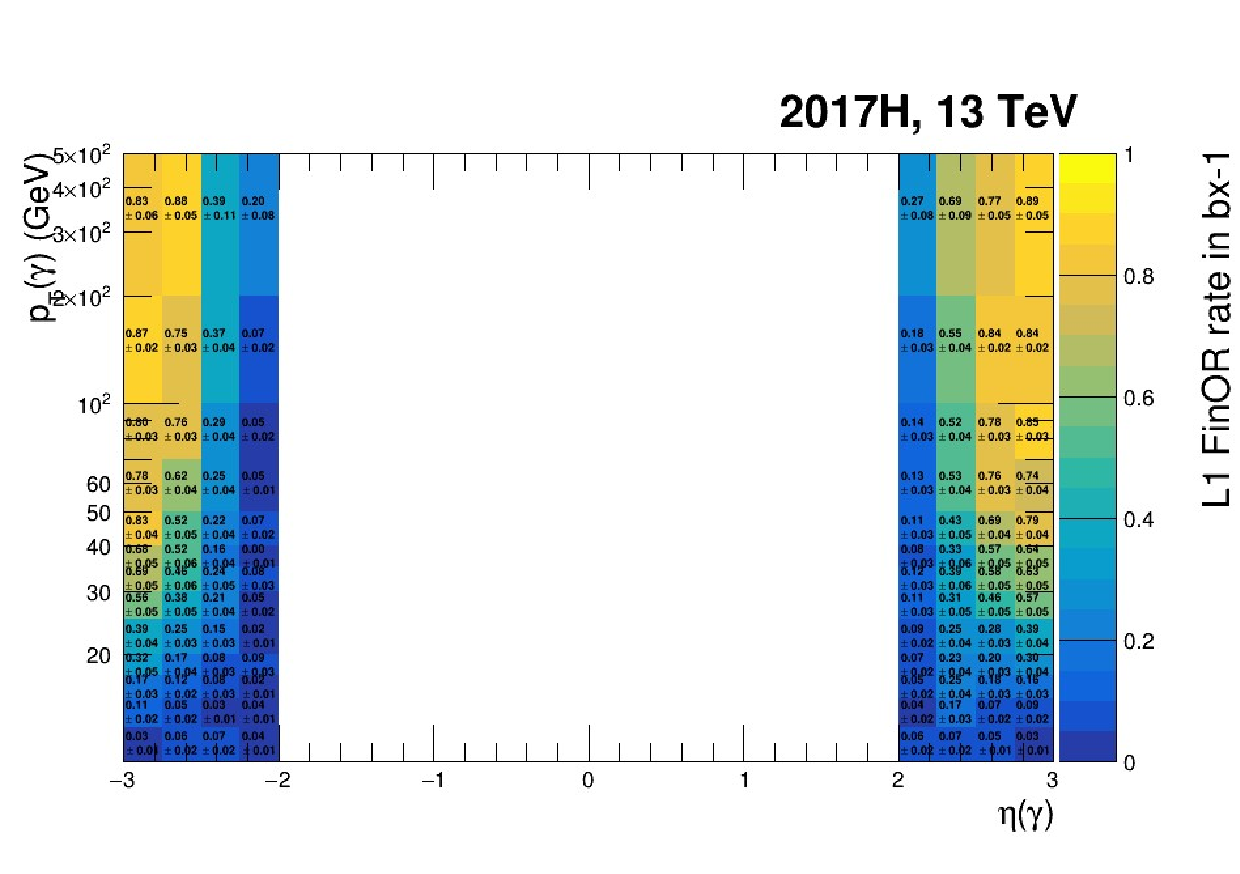
\includegraphics[width=0.49\textwidth]{plots/Prefire/L1prefiring_photonpt_2017H.pdf}
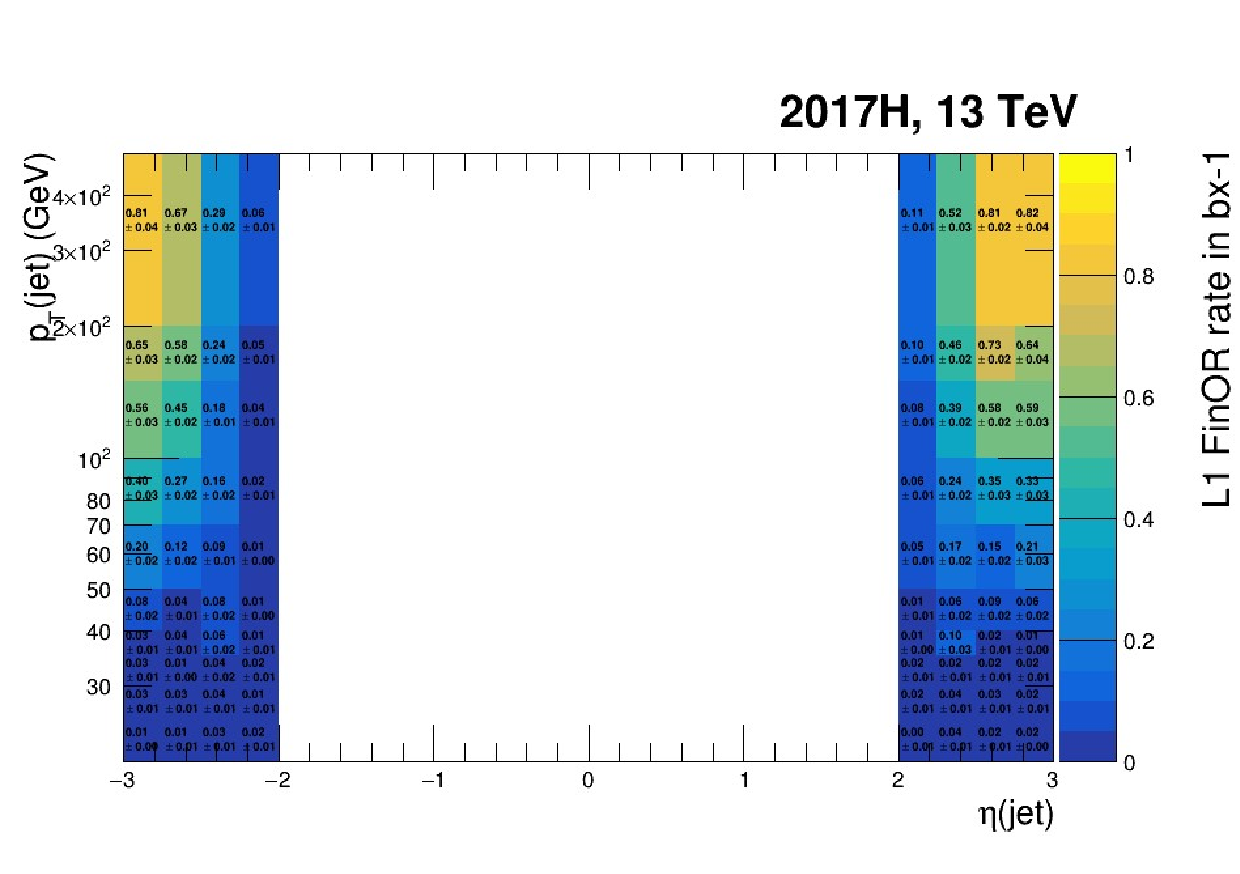
\includegraphics[width=0.49\textwidth]{plots/Prefire/L1prefiring_jetpt_2017H.pdf}
\caption{Pre-firing probability maps for photons (left) and jets (right) for 2017H (\sh). The $z-\mathrm{axis}$ represents the probability of an object with $(\pt,\eta)$ causing pre-firing. Objects with higher \pt and $|\eta| \sim 3$ are more likely to cause pre-firing. Objects with $|\eta| < 2$ do not cause pre-firing.}
\label{fig:prefire:2017H}
\end{figure}
\begin{equation}
    w_{pref} = 1 - P(\mathrm{prefire}) = \prod_{i=\gamma,jets}{(1 - \epsilon_i^{pref}(\eta,p_T))}
    \label{eq:prefiring_weight}
\end{equation}
Prefiring probability maps for jets and photons are shown in Figure~\ref{fig:prefire:2017G} for 2017G (\sg) and Figure~\ref{fig:prefire:2017H} for 2017H (\sh). Trigger rules can be exploited to make a selection of "un-prefireable" events to serve as the baseline measurement to quantify the prefiring rate, which consist of events in BX0 with an event in BX-3 accepted by the L1 trigger. The rate of prefiring is derived from a tag-and-probe method requiring a central tag and forward probe to ensure the probe is the source of the prefiring.  Photon prefiring probability is derived from the single electron trigger dataset and the jet prefiring probability is derived from the single muon trigger dataset. In Equation~\ref{eq:prefiring_weight}, the probability of prefiring due to an individual photon or jet given its \pt and $\eta$ is $\epsilon_i^{pref}(\eta,p_T)$. In events with overlapping photons and jets (with $\Delta  R < 0.4$), only the contribution from the object with the highest probability of prefiring is used in Equation~\ref{eq:prefiring_weight}\cite{LATHOMAS}. Yield predictions from the \Wpm and \Z boson signal simulation are re-normalized to account for the prefiring effect, with correction factors listed in Table~\ref{tab:prefire:5} for 2017G (\sg) and Table~\ref{tab:prefire:13} for 2017H (\sh). Uncertainties in the prefiring probability are taken to be the maximum of the statistical uncertainty or 20\% of the prefiring probability. The effect of prefiring on the \zee rapidity distribution for 2017G (2017H) is shown in  Figure~\ref{fig:prefire:zrap:2017G} (Figure~\ref{fig:prefire:zrap:2017H}). These figures also demonstrate the effectiveness of the corrections at mitigating the effects of prefiring on forward events.
\begin{figure}[htb]
\centering
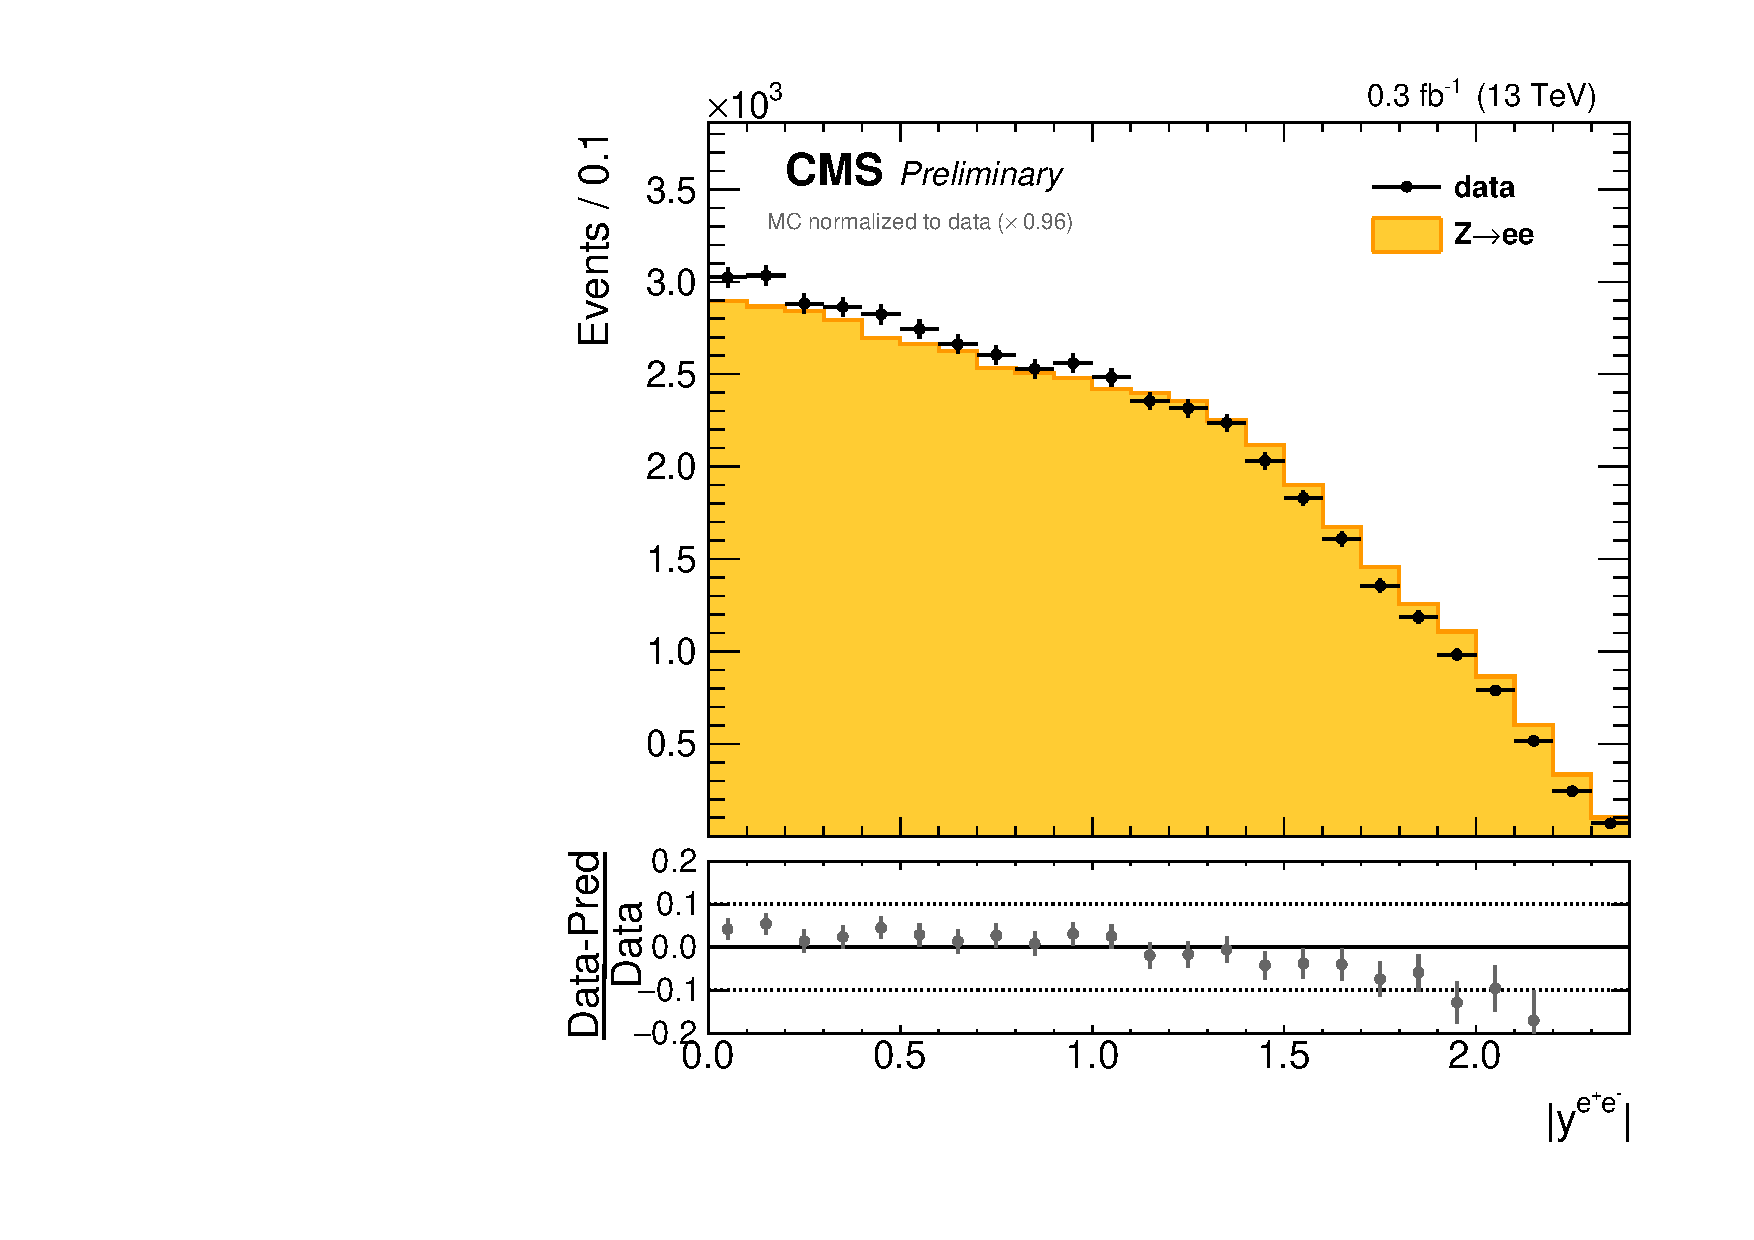
\includegraphics[width=0.49\textwidth]{plots/Prefire/Zee5_Zrap_noPrefire.pdf}
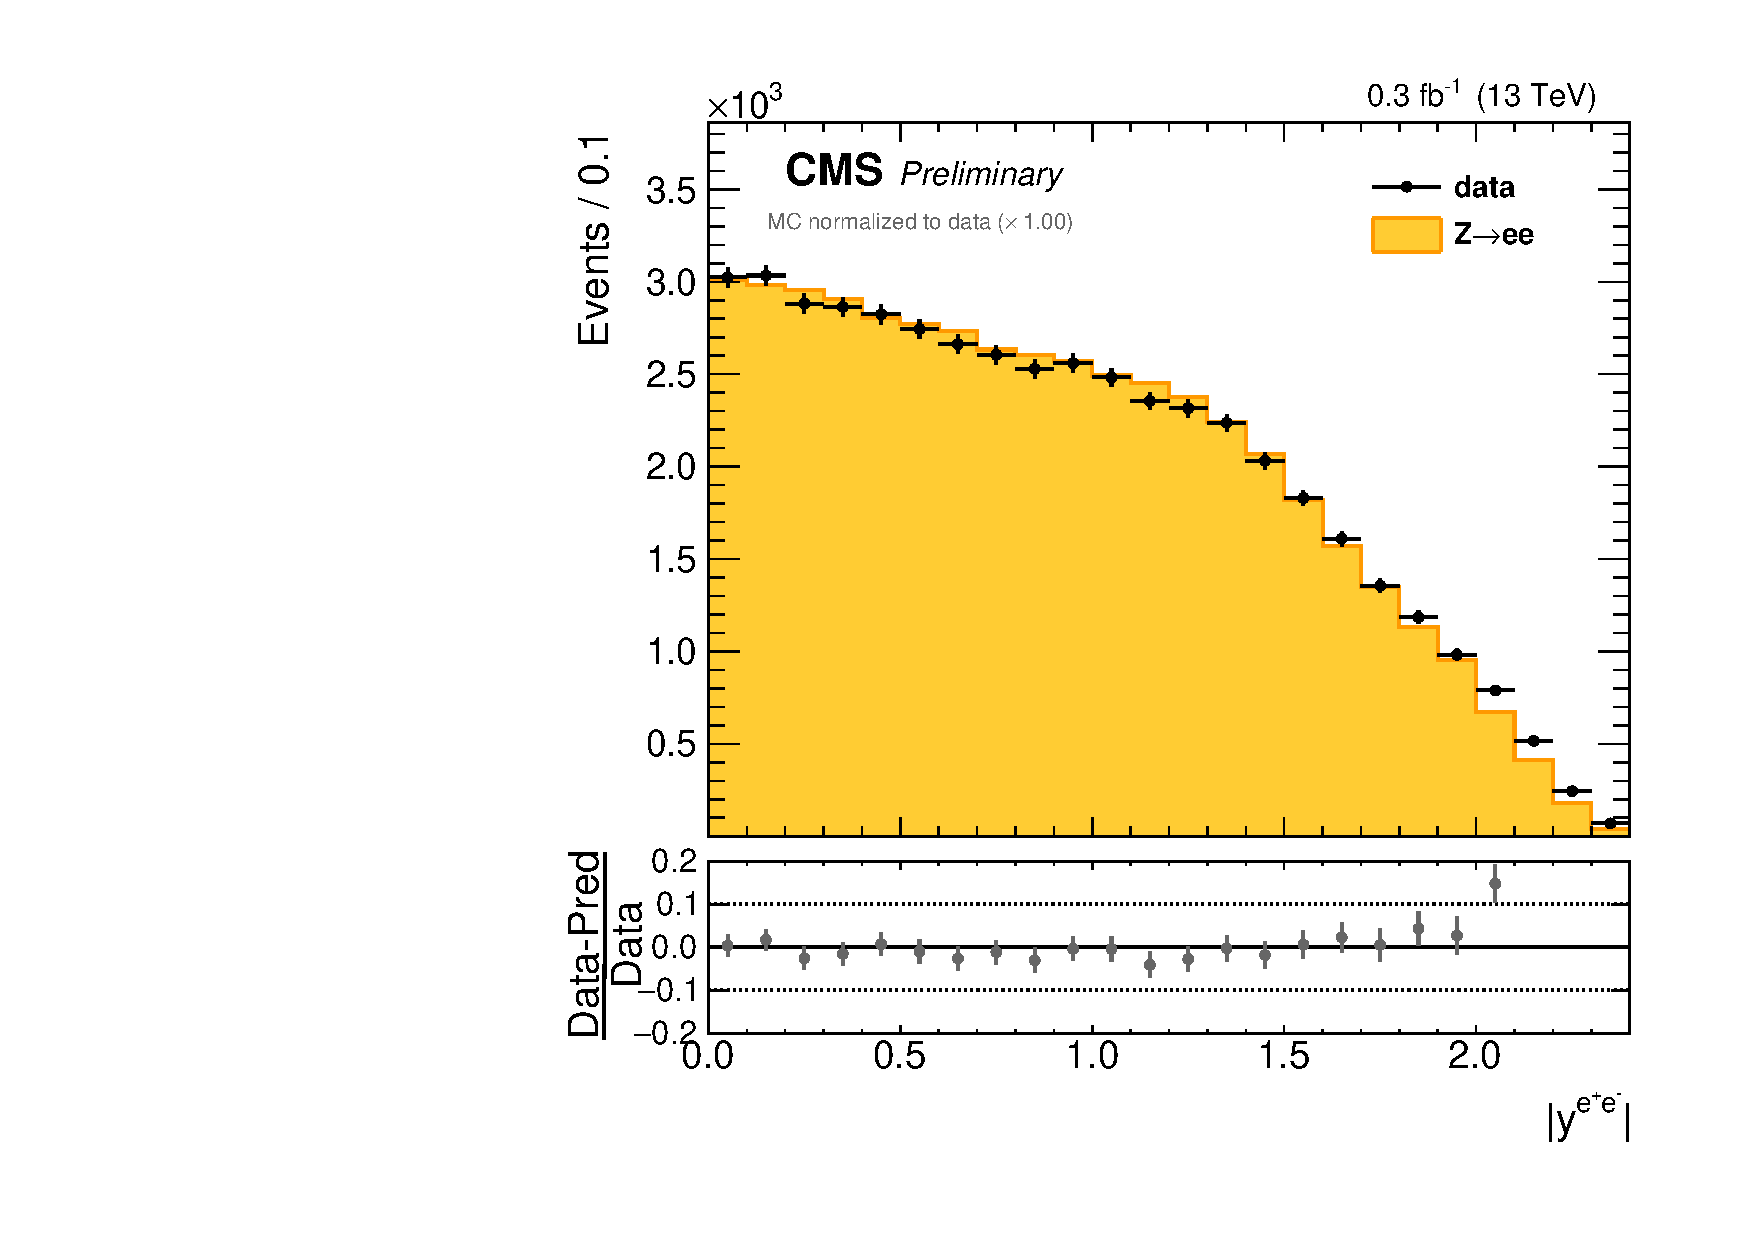
\includegraphics[width=0.49\textwidth]{plots/Prefire/Zee5_Zrap_inclPrefire.pdf}
\caption{\zee rapidity before (left) and after (right) pre-firing corrections, 2017G (\sg).}
\label{fig:prefire:zrap:2017G}
\end{figure}

\begin{figure}[htb]
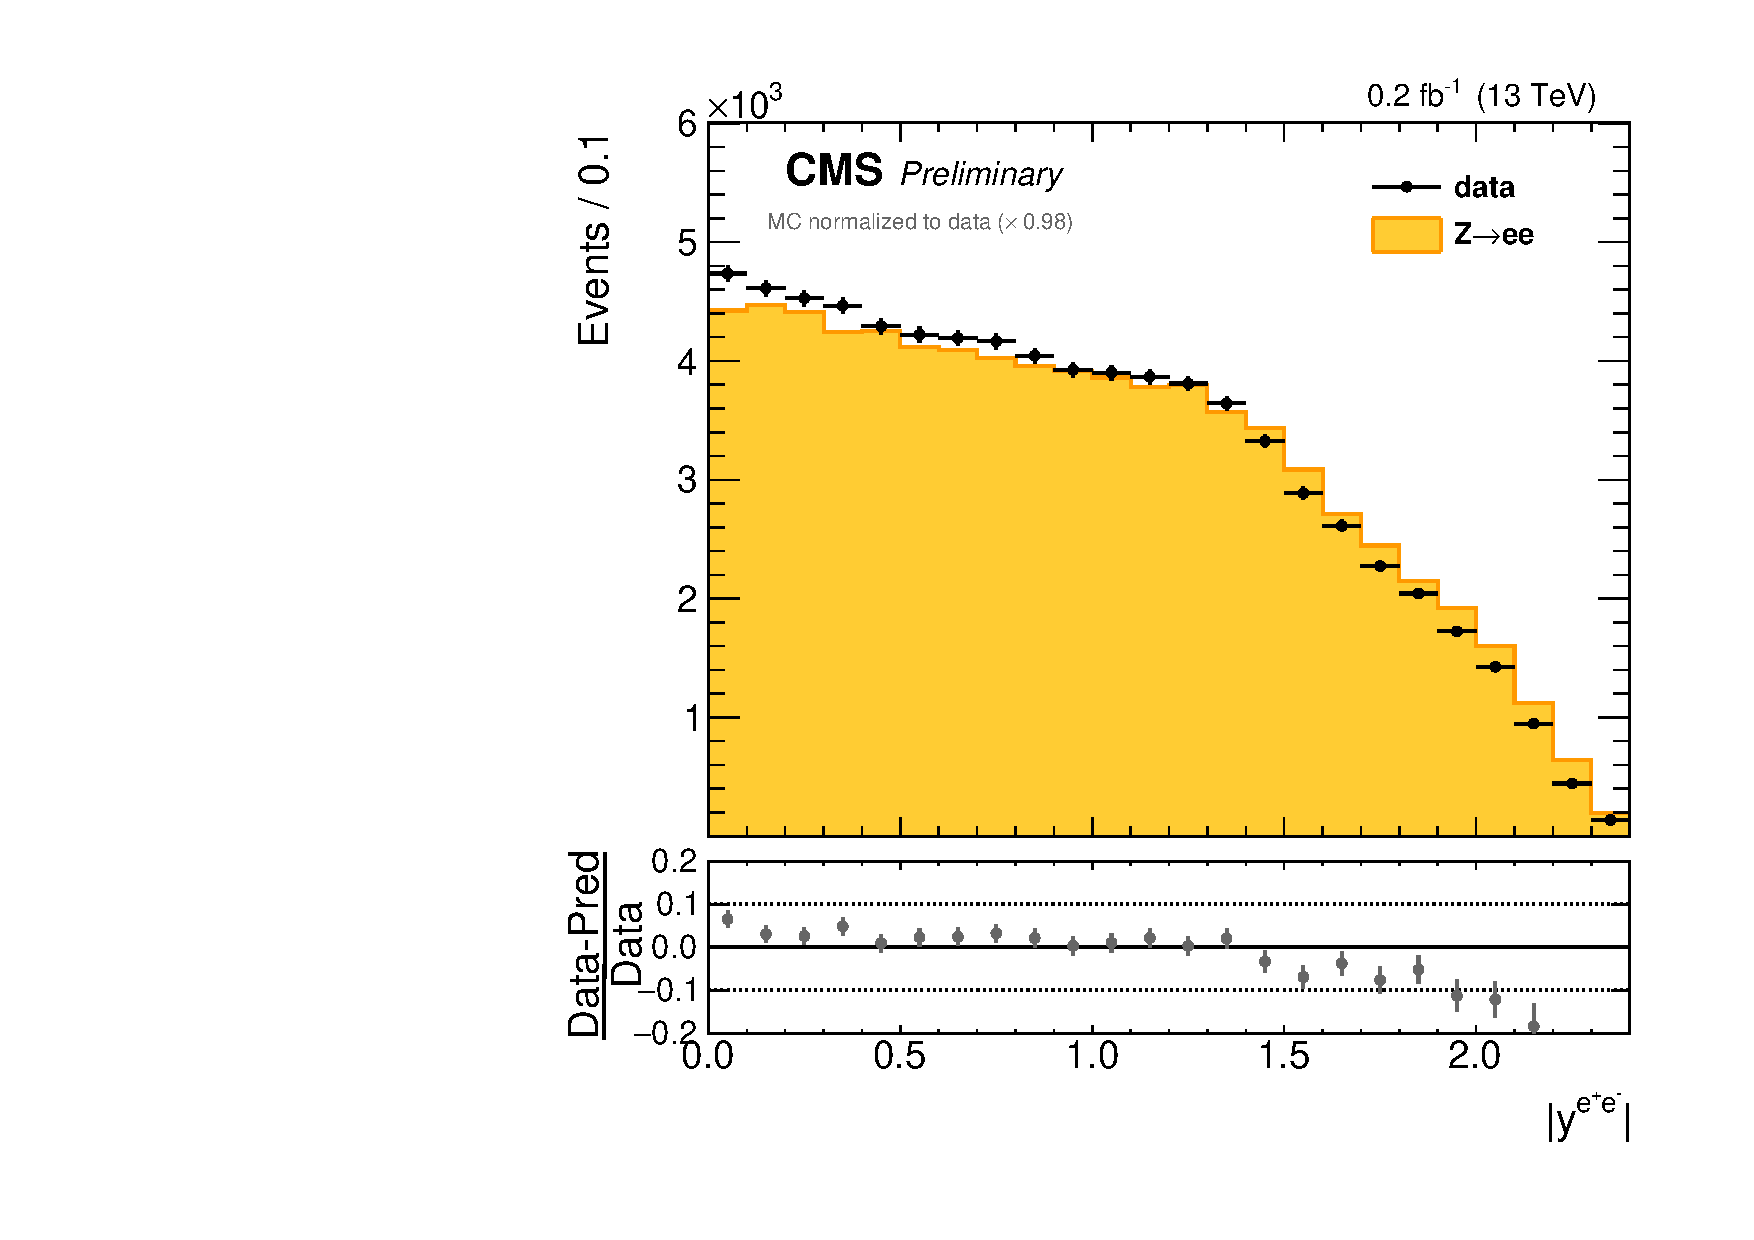
\includegraphics[width=0.49\textwidth]{plots/Prefire/Zee13_Zrap_noPrefire.pdf}
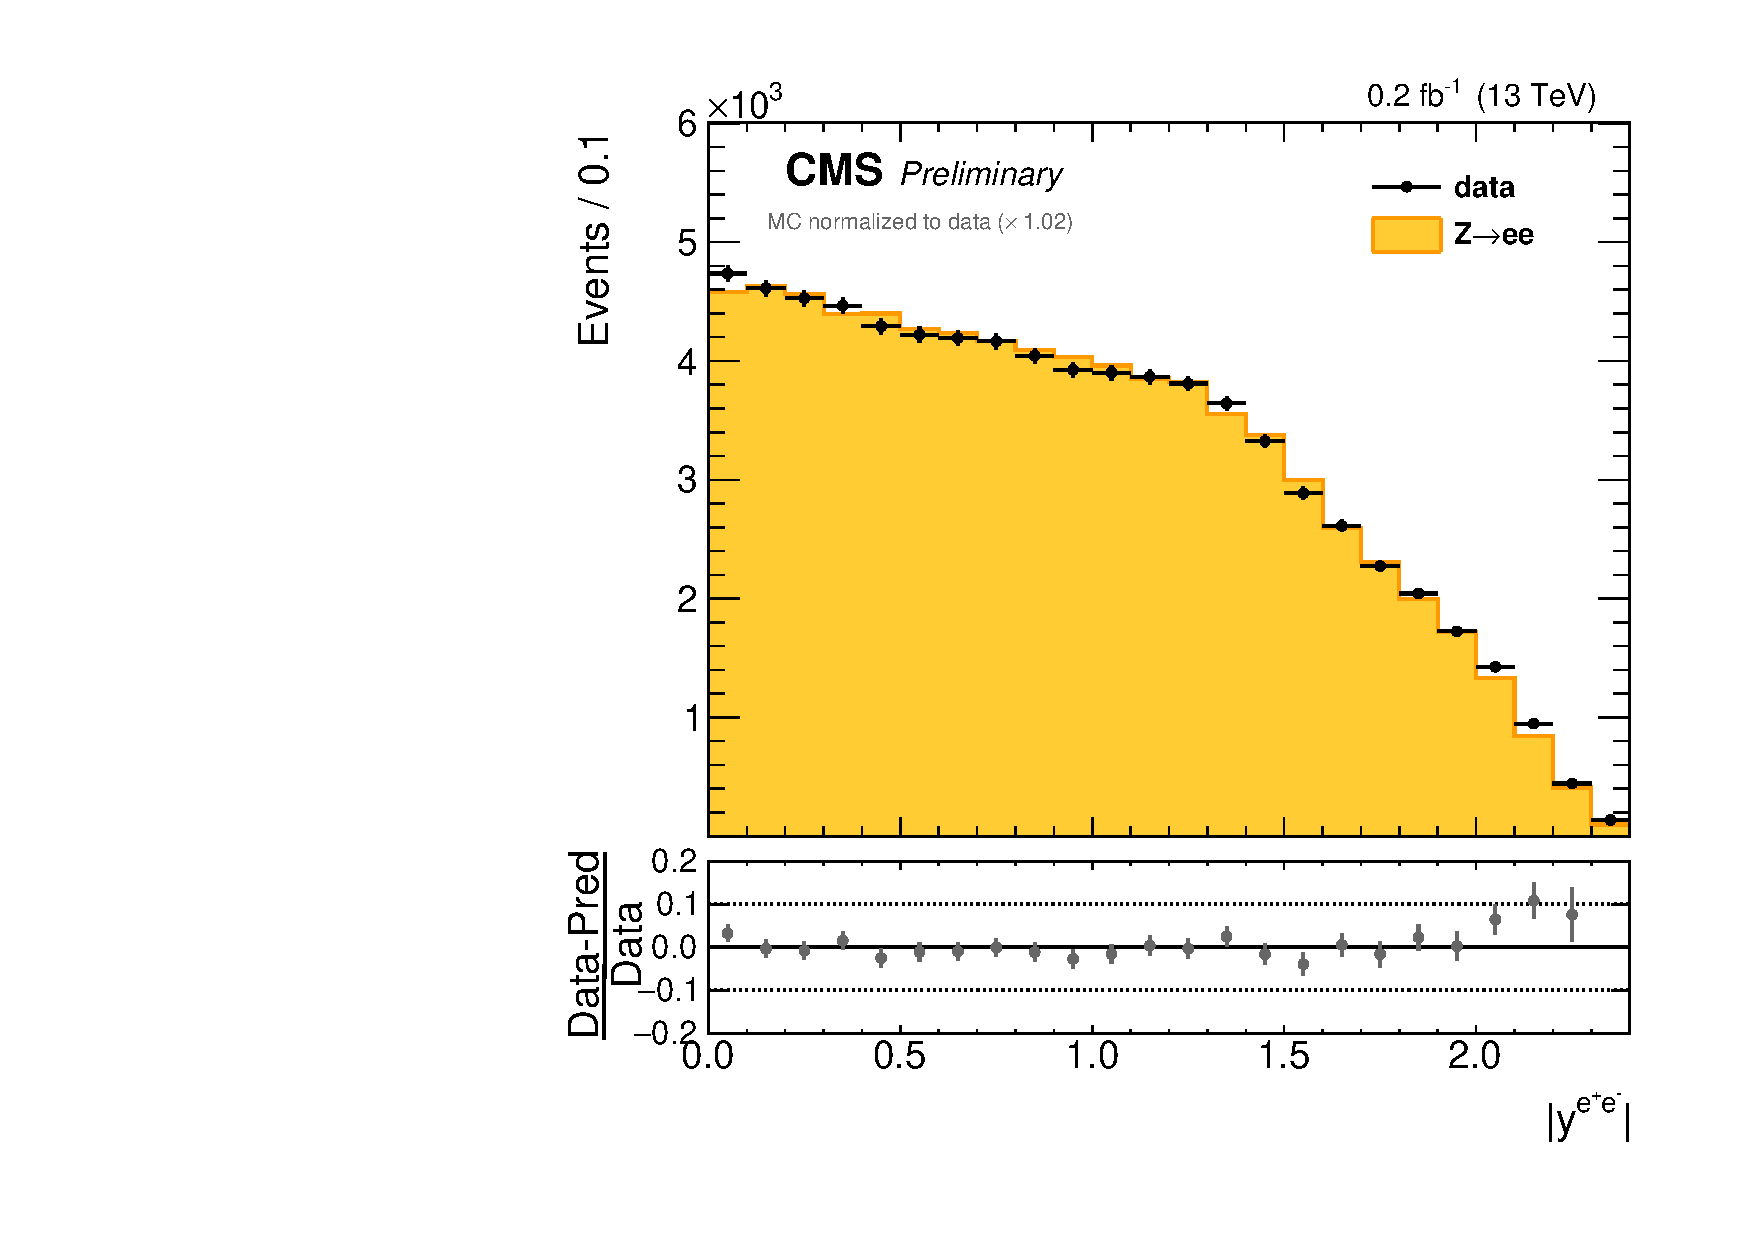
\includegraphics[width=0.49\textwidth]{plots/Prefire/Zee13_Zrap_inclPrefire.pdf}
\caption{\zee rapidity before (left) and after (right) pre-firing corrections, 2017H (\sh).}
\label{fig:prefire:zrap:2017H}
\end{figure}
%%%% Table containing prefire effects, 5 TeV
\begin{table}[htbp]
\begin{center}
\begin{tabular}{|c|c|c|c|c|}
\hline
Process & Jets & Photons & Total \\\hline \hline
$W\rightarrow e^+\nu$      & 0.990 & 0.977 & 0.975 \\
$W\rightarrow e^-\nu$      & 0.990 & 0.978 & 0.976 \\
$Z\rightarrow ee$          & 0.986 & 0.961 & 0.959 \\
\hline
$W\rightarrow \mu^+\nu$   & 0.989 & 0.998 & 0.988 \\
$W\rightarrow \mu^-\nu$   & 0.989 & 0.999 & 0.989\\
$Z\rightarrow \mu\mu$     & 0.985 & 0.999 & 0.985 \\
\hline
\end{tabular} 
\end{center}


\caption{Impact of prefiring on the reconstruction efficiency of each of the \Wp, \Wm, and \Z boson channels for the \sg (2017G) dataset. Corrections are applied differentially and table reports total efficiency integrated over full phase space. The "Total" column includes proper counting of overlapping objects and is the total efficiency scale factor due to pre-firing.}
\label{tab:prefire:5}
\end{table}

%%%% Table containing prefire effects, 13 TeV
\begin{table}[htbp]
\begin{center}
\begin{tabular}{|c|c|c|c|c|}
\hline
Process & Jets & Photons & Total \\\hline \hline
$W\rightarrow e^+\nu$      & 0.989 & 0.970 & 0.967 \\
$W\rightarrow e^-\nu$      & 0.990 & 0.974 & 0.971\\
$Z\rightarrow ee$          & 0.988 & 0.964 & 0.962 \\
\hline
$W\rightarrow \mu^+\nu$   & 0.990 & 0.996 & 0.988 \\
$W\rightarrow \mu^-\nu$   & 0.991 & 0.997 & 0.989 \\
$Z\rightarrow \mu\mu$     & 0.989 & 0.997 & 0.987 \\
\hline
\end{tabular}
\end{center}

\caption{Impact of prefiring on the reconstruction efficiency of each of the \Wp, \Wm, and \Z boson channels for the \sh (2017H) dataset. The "Total" column includes proper counting of overlapping objects and is the scale factor by which the expected number of events is adjusted.}
\label{tab:prefire:13}
\end{table}
